\documentclass[hyperref={pdfpagelabels=false},table,9pt,compress]{beamer}     %mathserif,
% File Name: SetUp.tex
% Function: Make main settings of the document.


%%%%%%%%%%%%%%%%%%%%%%%%%%% BEGIN-Theme-settings %%%%%%%%%%%%%%%%%%%%%%%%%%
%%%%% http://www.hartwork.org/beamer-theme-matrix/
\usetheme{default} % Set the theme of the beamer.
%\usetheme{Frankfurt}                     %% Geovani style
%\setbeamercolor{alerted text}{fg=blue}   %% Geovani style
% W/o������:default, boxes, Bergen, Madrid, Pittsburgh, Rochester
% ���������:Antibes, JuanLesPins, Montpellier��
% ��Ŀ¼(TOC)�IJ�ߵ�����: Berkeley, PaloAlto, Goettingen, Marburg, Hannover��
% ��΢��frame������:Berlin, Ilmenau, Dresden, Darmstadt, Frankfurt, Singapore, Szeged��
% ����С�ڱ���: Copenhagen, Luebeck, Malmoe, Warsaw��
%\usecolortheme{default}  % Outer color themes. Alternatives: whale, seahorse, dolphin. default, beaver
\usecolortheme{orchid}  % Inner color themes. Alternatives: lily, orchid.
\useinnertheme[shadow]{rounded}
\usefonttheme{structurebold} % Font themes. Alternatives:  default, serif, structurebold, structureitalicserif, structuresmallcapsserif
\setbeamertemplate{frametitle}
{   \begin{center}
        \insertframetitle
    \end{center}
}
\setbeamertemplate{itemize items}[default] % Alternatives: default/triangle, circle, square, ball
\setbeamertemplate{enumerate items}[default] % Alternatives: default, circle, square, ball
\setbeamertemplate{navigation symbols}{}
\setbeamertemplate{footline}[frame number]
%\setbeamertemplate{footline}{%
%  \leavevmode%
%  \hbox{%
%    \begin{beamercolorbox}[wd=.333333\paperwidth,ht=2.25ex,dp=1ex,center]{author in head/foot}%
%      \usebeamerfont{author in head/foot}\insertshortauthor~(\insertshortinstitute)
%    \end{beamercolorbox}%
%    \begin{beamercolorbox}[wd=.333333\paperwidth,ht=2.25ex,dp=1ex,center]{title in head/foot}%
%      \usebeamerfont{title in head/foot}\insertshorttitle
%    \end{beamercolorbox}%
%    \begin{beamercolorbox}[wd=.333333\paperwidth,ht=2.25ex,dp=1ex,right]{date in head/foot}%
%      \usebeamerfont{date in head/foot}\insertshortdate{}\hspace*{2em}
%      \insertframenumber{} / \inserttotalframenumber \hspace*{2ex}
%    \end{beamercolorbox}
%    }%
%  \vskip0pt%
%}
%%%%%%%%%%%%%%%%%%%%%%%%%%%% END-Theme-settings %%%%%%%%%%%%%%%%%%%%%%%%%%%


%%%%%%%%%%%%%%%%%%%%%%%%%%%%%% BEGIN-Packages %%%%%%%%%%%%%%%%%%%%%%%%%%%%%
\usepackage{amsmath,amssymb,amsfonts}
\usepackage{mathrsfs}
\usepackage{color,xcolor}
\usepackage{graphicx,subfigure}
\usepackage{clock} % Use this package to insert a clock in the beamer.
\usepackage{textcomp}
\usepackage[T1]{fontenc}
\usepackage{verbatim}
\usepackage{moreverb}
\usepackage{multirow,multicol}
%\usepackage{url}
%\usepackage[colorlinks,linkcolor=blue,citecolor=blue,urlcolor=blue]{hyperref}%[colorlinks,linkcolor=blue,citecolor=blue,urlcolor=blue]
\usepackage{CJK}
%%%%%%%%%%%%%%%%%%%%%%%%%%%%%%%% END-Packages %%%%%%%%%%%%%%%%%%%%%%%%%%%%%


% \setbeamertemplate{navigation symbols}{} % Disable the buttons at the bottom.

\graphicspath{{Figures/}} % Set the directory where figures are saved.

%\AtBeginSection{
%  \begin{frame}{Outline}
%    \tableofcontents[currentsection,hideallsubsections]
%  \end{frame}
%}
%\AtBeginSubsection{
%  \begin{frame}{Outline}
%    \tableofcontents[currentsection,currentsubsection]
%  \end{frame}
%}
\AtBeginSection{
  \begin{frame}{Outline}
  \large{
  \tableofcontents[sections={\thesection}]  }
  \end{frame}
}

%%%%%%%%%%%%%%%%%%%% BEGIN-Theorem-like Environments %%%%%%%%%%%%%%%%%%%%%
\newtheorem{mybox}{}
\newtheorem{Con}{Conjecture}[section]
\newtheorem{Thm}{Theorem}[section]
\newtheorem{Prop}{Proposition}[Thm]
% show fig and table number
\setbeamertemplate{caption}[numbered]
% show theorems and example number
\setbeamertemplate{theorems}[numbered]
%%%%%%%%%%%%%%%%%%%%% END-Theorem-like Environments %%%%%%%%%%%%%%%%%%%%%%


%%%%%%%%%%%%%%%%%%%%%%%%%% BEGIN-New Commands %%%%%%%%%%%%%%%%%%%%%%%%%%%%
\newcommand{\email}[1]{Email: \href{mailto: #1}{\tt {\color{blue}#1}}}
\newcommand{\red}{\color{red}}
\newcommand{\blue}{\color{blue}}
\newcommand{\brown}{\color{brown}}
\newcommand{\orange}{\color{orange}}
\newcommand{\yellow}{\color{yellow}}
\newcommand{\Real}{\mathbb{R}}
\newcommand{\Tran}[1]{#1^\mathrm{T}}
\newcommand{\st}{\textnormal{s.t.}}
\newcommand{\dist}{\textnormal{dist}}
\newcommand{\bc}{\begin{center}}
\newcommand{\ec}{\end{center}}
\newcommand{\tbf}{\textbf}
\newcommand{\be}{\begin{equation}}
\newcommand{\ee}{\end{equation}}
\newcommand{\ba}{\begin{array}}
\newcommand{\ea}{\end{array}}
\newcommand{\btab}{\begin{table}\begin{tabular}}
\newcommand{\etab}{\end{tabular}\end{table}}
\newcommand{\nn}{\nonumber}
\newcommand{\xn}{x_1,x_2,\ldots,x_n}
\newcommand{\framee}[2]{\frame{\frametitle{#1} #2}}
\newcommand{\reff}[1]{(\ref{#1})} % ������
\newcommand{\inner}[2]{\left\langle#1,#2\right\rangle}

%\renewcommand{\baselinestretch}{1.3}
% Ĭ��������룬������ó����˶���
\renewcommand{\raggedright}{\leftskip=0pt \rightskip=0pt plus 0cm}
\raggedright
%\large
% define Roman numbers
\makeatletter
\newcommand{\rmnum}[1]{\romannumeral #1}
\newcommand{\Rmnum}[1]{\expandafter\@slowromancap\romannumeral #1@}
\makeatother
%%%%%%%%%%%%%%%%%%%%%%%%%%%% END-New Commands %%%%%%%%%%%%%%%%%%%%%%%%%%%%

\usepackage[ruled]{algorithm2e}

\begin{document}
\begin{CJK*}{GBK}{kai}

\title[distance geometry]{\textsc{A New Error Function and Its Application in Distance Geometry Problem}}
\author[Zhenli SHENG]{Zhenli Sheng (ʢ����)\\email: {\blue szl@lsec.cc.ac.cn}}
% \institute{Institute of Computational Mathematics and Scientific/Engineering Computing}
\institute[ICMSEC, CAS]{Institute of Computational Mathematics and Scientific/Engineering Computing,\\Chinese Academy of Sciences}
\date[]{joint work with {\blue Prof. Ya-xiang Yuan} \\\textrm{} \\January 8, 2013\\ seminar talk}
\frame{
\titlepage
}

% File Name: ThankYou.tex
% Function: Insert an Outline page.


%\section*{\textsc{Outline}}
%\begin{frame}
%\frametitle{\textsc{Outline}}
%\end{frame}

\begin{frame}
\frametitle{\textsc{Outline}}
\tableofcontents%[pausesections]
\end{frame}


\section{Problem introduction}
\frame{
\frametitle{Distance Geometry Problem}
Find the coordinate vectors $x_{1},x_{2},\ldots,x_{n}$ that satisfy several given distances among them. Mathematically, this problem can be stated as following, \\
\vspace{0.5cm}
\red{
Find $x_{1},x_{2},\ldots,x_{n}$, such that
\begin{displaymath}
\|x_{i}-x_{j}\|=d_{ij},\quad (i,j) \in S.
\end{displaymath}
or
\begin{displaymath}
l_{ij}\leq \|x_{i}-x_{j}\|\leq u_{ij},\quad (i,j) \in S.
\end{displaymath}
}
\begin{itemize}
  \item The data given may have some errors.
  \item This problem can be formulated as a global optimization problem.
  \item It has many applications.
\end{itemize}
}

\frame{
\frametitle{Application \Rmnum{1}: Graph Realization}
\begin{figure}
  \centering
  \subfigure{ 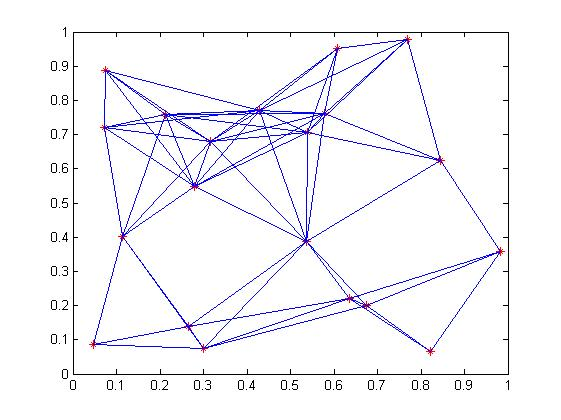
\includegraphics[width=5cm]{GraphRealization.jpg} }
  \subfigure{ 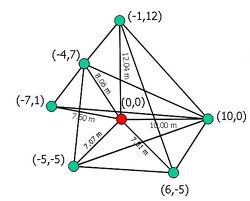
\includegraphics[width=5cm]{GraphRealization2.jpg} }
  \caption{ Graph Realization in 2D}
\end{figure}
\begin{center}
  Given a graph G=(V,E), each edge has a weight.
\end{center}
}

\frame{
\frametitle{Application \Rmnum{2}: Protein Structure Determination}
\begin{figure}[htp]
    \centering
    \subfigure{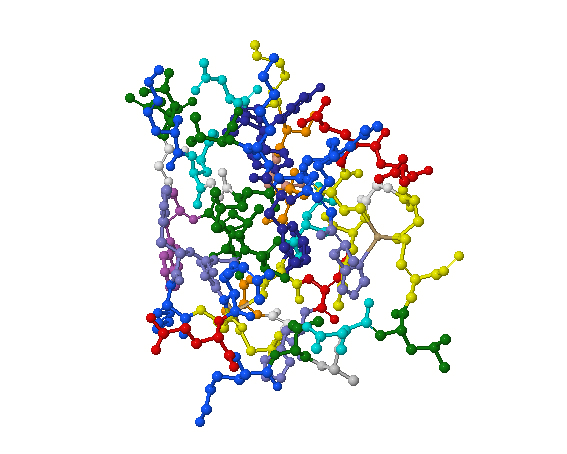
\includegraphics[width=5cm]{1PTQ2.jpg} }
    \subfigure{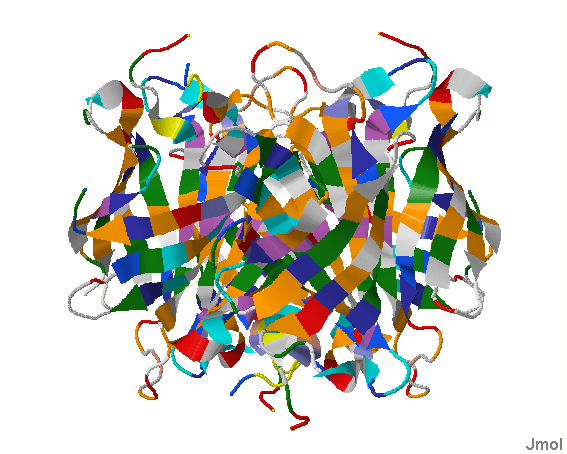
\includegraphics[width=5cm]{1HQQ2.jpg} }
    \caption{Two proteins: 1PTQ and 1HQQ, in different display ways}
\end{figure}
\begin{center}
  Measure distances: NMR, X ray crystallography.
\end{center}
}

\frame{
\frametitle{Application \Rmnum{3}: Sensor Network Localization}
\begin{figure}[htp]
    \centering
    \subfigure{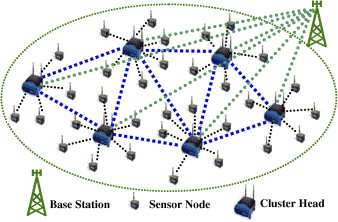
\includegraphics[width=4.5cm]{sensor2.jpg} }
    \subfigure{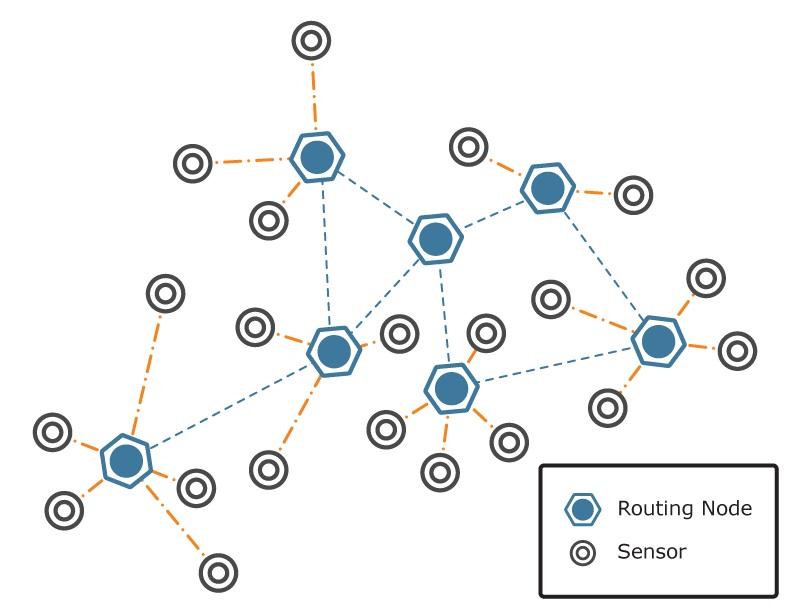
\includegraphics[width=4.5cm]{sensor1.jpg} }
    \caption{Illustration of wireless sensor networks: anchor and sensor}
\end{figure}
}

\section{Related works review}
\subsection{Matrix decomposition method}
\frame{
\frametitle{Matrix Decomposition Method}
{\blue Matrix decomposition method [Blumenthal 1953, Torgerson 1958]} works for {\red Distance Geometry problem with full set of exact distances.} \\
%\textrm{}\\
\small{
Given a full set of distances, $d_{ij} = \| x_{i}-x_{j} \|, \quad i,j=1,2,\ldots,n.$ \\
\begin{itemize}%[$\blacktriangleright$]
  \item Set $x_{n} = (0,0,0\Tran)$, thus $d_{in}=\|x_i\|$, we have
      \begin{eqnarray}
      % \nonumber to remove numbering (before each equation)
        \nonumber d_{ij}^{2} &=& \|x_{i}-x_{j}\|^{2} \\
        \nonumber             &=& \|x_{i}\|^{2}-2\Tran x_{i} x_{j}+\|x_{j}\|^{2} \\
                              &=& d_{in}^{2}-2\Tran x_{i} x_{j}+d_{jn}^{2}, \qquad  i,j=1,2,\ldots,n-1 \label{eq1}
      \end{eqnarray} \\
      \textrm{}\\
  \item Define $ X=(x_{1},x_{2},\ldots,x_{n}\Tran)$ and $D=\{(d_{in}^{2}-d_{ij}^{2}+d_{jn}^{2})/2: i,j=1,2,\ldots,n-1\}$,  (\ref{eq1}) $\Rightarrow {\red X\Tran X=D}$.\\
      \textrm{}\\
  \item Let $D=U\Sigma\Tran U$, $V=U(:,1:3)$ and $\Lambda=\Sigma(1:3,1:3)$. Then $X = V\Lambda^{1/2}$ is the best rank-3 approximation. [{\blue Eckart-Young 1936}]
\end{itemize} }
}


\subsection{Buildup method}
\frame{
\frametitle{Buildup Method}
\begin{algorithm}[H]
\vspace{0.3cm}
Given: distance matrix D.
\begin{enumerate}[Step 1:]
  \item Find a clique of four points and determine their coordinates.
  \item Choose a point to be added, apply liner or nonlinear least square to locate the point.
  \item Repeat {\blue Step 2} until all points are determined or no more points can be determined.
\end{enumerate}
\caption{Buildup Method for Distance Geometry Problem with sparse data}
\end{algorithm}
\vspace{0.5cm}
$\spadesuit$ It was first proposed by {\blue [Dong-Wu 2002]}. We will specify details of each step later.
}

\frame{
\frametitle{Determine first four points}
\begin{itemize}
  \item Find a clique of four points: we simply exploit greedy method
  \item How to determine their coordinates? \\
       Denote $x_{i} = (u_{i},v_{i},w_{i}\Tran)$, set $x_{1}=(0,0,0\Tran)$ and $x_{2}=(d_{12},0,0\Tran)$.
        \begin{displaymath}
        \setlength\arraycolsep{1pt}
        \left\{\begin{array}{rcl}
        u_{3}^{2} + v_{3}^{2} &=& d_{31}^{2} \\
        (u_{3}-u_{2})^{2} + v_{3}^{2} &=& d_{32}^{2}
        \end{array} \right.
        \Rightarrow
        \left\{\begin{array}{rcl}
        u_{3} &=& (d_{31}^{2}-d_{32}^{2}+u_{2}^{2})/(2u_{2}) \\
        v_{3} &=& {\blue \sqrt{d_{31}^{2}-u_{3}^{2}}}, \quad w_3=0
        \end{array} \right.
        \end{displaymath}
        \begin{displaymath}
        \setlength\arraycolsep{1pt}
        \left\{ \begin{array}{rcl}
        u_{4}^{2} + v_{4}^{2} + w_{4}^{2} &=& d_{41}^{2} \\
        (u_{4}-u_{2})^{2} + v_{4}^{2} + w_{4}^{2} &=& d_{42}^{2} \\
        (u_{4}-u_{3})^{2} + (v_{4}-v_3)^{2} + w_{4}^{2} &=& d_{43}^{2}
        \end{array} \right.
        \Rightarrow
        \left\{\begin{array}{rcl}
        u_{4} &=& (d_{41}^{2}-d_{42}^{2}+u_{2}^{2})/(2u_{2}) \\
        v_{4} &=& ... \\
        w_{4} &=& {\blue \sqrt{d_{41}^{2}-u_{4}^{2}-v_{4}^{2}}}
        \end{array} \right.
        \end{displaymath}
        $v_{4} = (d_{42}^{2}-d_{43}^{2}+(u_{4}-u_{2})^{2}+(u_{4}-u_{3})^{2}+v_{3}^{2})/(2v_{3})$
  \item In the noisy case, the {\blue "sqrt"} part may cause problems.
\end{itemize}
}

\frame{
\frametitle{Which point to be chosen?}
\begin{itemize}
  \item Computational order
  \item Greedy strategy: choose the point which has the most known distances to the determined points
  \item Symmetric Reverse Cuthill-McKee order: MATLAB {\blue symrcm}\\
     minimize the bandwidth $= \max \{|i-j| : d_{ij}\neq 0\}$
\begin{figure}
  \centering
  \subfigure{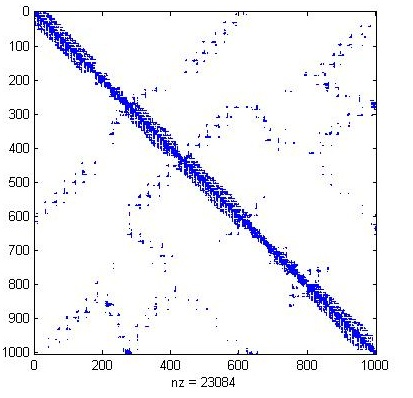
\includegraphics[width=0.3\textwidth]{1AX8original.jpg}}
  \subfigure{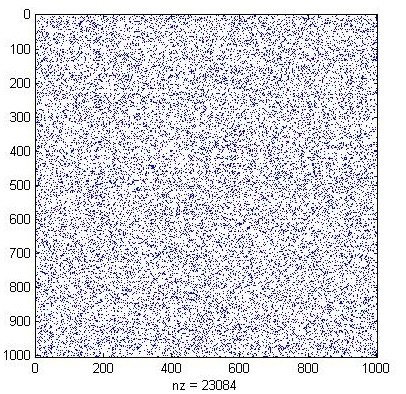
\includegraphics[width=0.3\textwidth]{1AX8randperm.jpg}}
  \subfigure{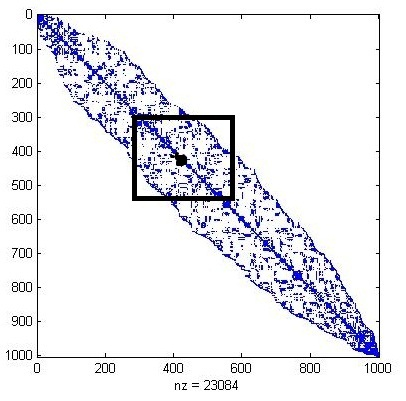
\includegraphics[width=0.3\textwidth]{1AX8symrcm.jpg}}
  \caption{1AX8 distance matrix with different orders: original, randperm, symrcm}
\end{figure}
\end{itemize}
}

\frame{
\frametitle{Determine the chosen point}
Suppose $x_j$ (to be determined) has $l$ known distances with $x_i,x_2,\ldots,x_l$ (has been determined). \\
\begin{itemize}
  \item {\blue linear least square [Wu-Wu 2007]}��\\
  $d_{ij}^{2}=\|x_{i}\|^{2}-2\Tran x_{i} x_{j}+\|x_{j}\|^{2}, (i=1,2,\ldots,l). \Rightarrow {\red Ax_{j}=b},$ where \\
  $ \setlength\arraycolsep{2pt}
          A=2 \left(\begin{array}{ccc}
                    x_{11}-x_{21} & x_{12}-x_{22} & x_{13}-x_{23} \\
                    x_{21}-x_{31} & x_{22}-x_{32} & x_{23}-x_{33} \\
                    \vdots        & \vdots        & \vdots        \\
                    x_{l-1,1}-x_{l1} & x_{l-1,2}-x_{l2} & x_{l-1,3}-x_{l3} \\
                    \end{array} \right), $\\
  $        b= \left( \begin{array}{c}
                       (\|x_{1}\|^{2}- \|x_{2}\|^{2}) -( d_{1j}^{2}-d_{2j}^{2} )\\
                       (\|x_{2}\|^{2}- \|x_{3}\|^{2}) -( d_{2j}^{2}-d_{3j}^{2} )\\
                       \vdots                                                     \\
                       (\|x_{l-1}\|^{2}- \|x_{l}\|^{2}) -( d_{l-1,j}^{2}-d_{lj}^{2} )
                     \end{array}
         \right) $ \\
  \vspace{0.2cm}
  $\spadesuit$ In the noisy case, solve {\blue $\min_{x_j} \|Ax_j-b\|_2$}.
\end{itemize}
}

\frame{
\frametitle{Determine the chosen point}
Suppose $x_j$ (to be determined) has $l$ known distances with $x_1,x_2,\ldots,x_l$ (has been determined). \\
\begin{itemize}
\item {\blue nonlinear least square [Sit-Wu-Yuan 2009]}: \\
  \begin{enumerate}
    \item Calculate missing distances among these $l$ points.
    \item All the distances among $l+1$ points are known, we apply matrix decomposition method to solve it.
    \item Move these points back to the original reference system, using $x_i,x_2,\ldots,x_l$ as common points.
  \end{enumerate}
  $\clubsuit$ In this way, we determine the new point, while re-determine the $l$ points, which can be viewed as adjustment.
\end{itemize}
}

\frame{
\frametitle{Remarks about Buildup method}
\begin{itemize}
  \item Buildup method is almost perfect when the given distances are exact, as it is fast and accurate.
  \item Due to accumulation of round error, the result may damage if the number of the points is large (more than several thousands).
  \item Buildup method with nonlinear technique is more stable. However, it still can tolerate very small noise, usually no bigger than $0.01\%$.
\end{itemize}
}

\section{Our algorithm}
\frame{
\frametitle{Motivation}
Two facts:
\begin{itemize}
  \item It is almost impossible to find the global minimizer or a good local minimizer of any error function, from a randomly chosen initial point.
  \item Many existing methods can be casted into two parts:
  \begin{enumerate}[1)]
    \item Find a good initial point: \\
        {\blue Embedding Method [Crippen-Havel 1988]} trys to estimate the missing data, and then apply matrix decomposition method to obtain a solution. \\
        {\blue SDP Method [Biswas-Toh-Ye 2007]} solves a relaxed SDP problem to produce an initial point.
    \item Minimize an error function to adjust the positions. \\
        remark: these methods don't talk too much about this procedure, but actually it is very crucial to their methods.
  \end{enumerate}
\end{itemize}
}

\frame{
\frametitle{Our idea}
\begin{itemize}
  \item Incorporate Buildup Method and error function minimization.
  \item remark: \\ Buildup method is extremely fast, which is its most charming feature, but it cannot tolerate large noises, so we try to apply error minimization procedure to make it stable.
\end{itemize}

}

\frame{
\frametitle{How we come to the final algorithm}
\begin{itemize}
  \item At first, we try to adjust the recent $M$ points after every buildup step, so we choose \textbf{symrcm} order to implement buildup method. \\
       {\blue much better, still not so stable}
  \item Then, we add the $l$ points to this procedure.\\
   {\blue even better, but takes more time}
  \item Finally, I only use the $l$ points, and choose greedy order to implement buildup procedure. \\
       {\blue fantastic!}
\end{itemize}
}

\frame{
\frametitle{Our algorithm}
\begin{algorithm}[H]
\vspace{0.3cm}
Given: distance matrix D.
\begin{enumerate}[Step 1:]
  \item Find a clique of four points and determine their coordinates.
  \item Choose a point to be added, apply nonlinear least square to locate the point.
  \item {\red Apply error minimization to these $l+1$ points}.
  \item Repeat {\blue Step 2-3} until all points are determined or no more points can be determined.
  \item {\red Apply error minimization to all the determined points}.
\end{enumerate}
\caption{Buildup-based Error Minimization Method for Distance Geometry Problem with sparse and noisy distances}
\end{algorithm}
}

\subsection{Error function minimization}
\frame{
\frametitle{Error function minimization}
Currently, we simply use line search BB method to minimize the following error functions,
$$Stress(x_{1},x_{2},\ldots,x_{n}) = \sum_{(i,j)\in S} (\|x_{i}-x_{j}\|-d_{ij})^{2}$$
or
$$Yuan(x_{1},x_{2},\ldots,x_{n}) = \sum_{(i,j)\in S} h(\frac{\|x_{i}-x_{j}\|}{d_{ij}})$$
where
$$h(x) = \left\{ \begin{array}{ll}
                \frac{1}{2}(x-1)^2, & \textrm{if } x\geq 1, \\
                x-1-log(x),         & \textrm{if } 0<x<1.
                \end{array} \right.
$$
\vspace{0.3cm}
\begin{itemize}
  \item The effect are more or less the same.
  \item This is the most time-consuming part in our algorithm, which need to be further studied in the future work.
\end{itemize}
}

\frame{
\frametitle{Analysis of Stress function}
\begin{Thm}[Stress function]
Suppose $$f(x_{1},x_{2},\ldots,x_{n}) = \sum_{(i,j)\in S} \frac{1}{2}(\|x_{i}-x_{j}\|-d_{ij})^{2},$$ let $N(i)=\{j:d_{ij}\neq 0\}$ denote the neighbours of point $i$, and $x=(x_1;x_2;\dots;x_n)$ is a column vector in $\mathbb{R}^{3n}$, then we have
$$\frac{\partial f}{\partial x_i}=\sum_{j\in N(i)} (1-\frac{d_{ij}}{\|x_i-x_j\|})(x_i-x_j),$$
and for $k=1,2,3$,
$$\frac{\partial^2 f}{\partial x_{ik} \partial x_{jk}} = \renewcommand{\arraystretch}{1.1}
    \left\{ \begin{array}{rl}
    \sum\limits_{j\in N(i)}(\frac{d_{ij}(x_{ik}-x_{jk})^2}{\|x_i-x_j\|^3}+1-\frac{d_{ij}}{\|x_i-x_j\|}), & \textrm{if } i=j, \\
    -(\frac{d_{ij}(x_{ik}-x_{jk})^2}{\|x_i-x_j\|^3}+1-\frac{d_{ij}}{\|x_i-x_j\|}), & \textrm{if } j\in N(i), \\
    0, & \textrm{otherwise}.
    \end{array} \right.
$$
Then, 0 and $(1,1,\ldots,1\Tran)$ is an eigenpair. Furthermore, Hessian matrix is positive semidefinite at optimal point, and can be negative semidefinite otherwise.
\end{Thm}
}

\frame{
\frametitle{Analysis of Yuan function}
\begin{Thm}[Yuan function]
Suppose
$$
\begin{array}{ll}
f(x)&  = \sum\limits_{(i,j)\in S} h(\frac{\|x_i-x_j\|}{d_{ij}}) \\
 & =\sum\limits_{(i,j)\in S} \renewcommand{\arraystretch}{1.3}
 \left\{ \begin{array}{ll}
\frac{1}{2}(\frac{\|x_{i}-x_{j}\|}{d_{ij}}-1)^{2}, & \textrm{if } \|x_i-x_j\|\geq d_{ij}, \\
\frac{\|x_i-x_j\|}{d_{ij}} -1 -log(\frac{\|x_i-x_j\|}{d_{ij}}), & \textrm{otherwise}
\end{array} \right. \\
\end{array}
$$
the symbols are the same as those in the previous theorem, then we have
$$\frac{\partial f}{\partial x_i}=\sum_{j\in N(i)} \renewcommand{\arraystretch}{1.3}
\left\{ \begin{array}{ll}
(\frac{1}{d_{ij}^2}-\frac{1}{d_{ij}\|x_i-x_j\|})(x_i-x_j), & \textrm{if } \|x_i-x_j\|\geq d_{ij}, \\
(\frac{1}{d_{ij}\|x_i-x_j\|}-\frac{1}{\|x_i-x_j\|^2})(x_i-x_j), & \textrm{otherwise}
\end{array} \right.,$$
\end{Thm}
to be continued...
}

\frame{
\frametitle{Analysis of Yuan function(cont'd)}
\begin{Thm}[Yuan function]
and for $k=1,2,3$,
$$\frac{\partial^2 f}{\partial x_{ik} \partial x_{jk}} =
\left\{ \begin{array}{rl}
\sum\limits_{j\in N(i)}\omega(x), & \textrm{if } i=j, \\
-\omega(x),& \textrm{if } i\neq j, \\
0,         & \textrm{otherwise}
\end{array} \right. $$
where
$$\omega(x) = \renewcommand{\arraystretch}{1.5}
    \left\{ \begin{array}{ll}
    \frac{1}{d_{ij}^2} - \frac{1}{d_{ij}\|x_i-x_j\|} + \frac{(x_{ik}-x_{jk})^2}{d_{ij}\|x_i-x_j\|^3}, & \textrm{if } \|x_i-x_j\|\geq d_{ij}, \\
    \frac{1}{d_{ij}\|x_i-x_j\|}- \frac{1}{\|x_i-x_j\|^2}- \frac{(x_{ik}-x_{jk})^2}{d_{ij}\|x_i-x_j\|^3} + \frac{(x_{ik}-x_{jk})^2}{\|x_i-x_j\|^4}, & \textrm{otherwise}. \\
    \end{array} \right.
$$
Then, 0 and $(1,1,\ldots,1\Tran)$ is an eigenpair. Furthermore, Hessian matrix is positive semidefinite at optimal point, and can be negative semidefinite otherwise.
\end{Thm}
Proof. The positive semidefinite property follows by {\blue Gershgorin Circle Theorem}.
}

\frame{
\frametitle{Why we are better?}
\begin{itemize}
  \item We re-use the same distance information (but only the given distances, not include calculated ones).
  \item In Buildup method equipped with nonlinear least square, if distances are noisy, then we have
    $$\|x_{i}-x_{j}\|=d_{ij}+e_{ij},$$ where $e_{ij}$ denotes noise.
    $$\Rightarrow 2\Tran{x_i}x_j = d_{in}^2 - d_{ij}^2 + d_{jn}^2 {\blue - 2d_{ij}e_{ij} - e_{ij}^2}$$
  \item So, my conclusion is:\\
      {\red When the noises are large,} {\blue $(d_{ij}e_{ij} + e_{ij}^2/2)$} {\red should not be ignored, namely, solving $\Tran{X}X=D$ cannot give a very good solution to the original problem. But it can serve as a warm starting point to minimize an error function to obtain a better solution.}
\end{itemize}
}

\section{Numerical experiments}
\frame{
\frametitle{Numerical experiments}
We simulate on real protein structures, but the distance matrix is generated by us.\\
\begin{enumerate}
  \item Download PDB file from Internet to get the true positions of atoms.
  \item Use \emph{disk graph model} to generate distance matrix from these coordinates, with different cutoffs (6{\AA} or 5{\AA}) and variant noise level.
      $$d_{ij} = d_{ij} (1+noise*randn)$$
  \item Make numerical experiments with these distance matrices. {\blue Distances are the only information we need to implement our algorithm}.
  \item Examine the RMSD error of calculated positions with the true positions.
  $$ RMSD(X,Y) = \min_{Q,T}\{ \|X-YQ-T\|_{F}/\sqrt{n}: \Tran{Q}Q=I\} $$
\end{enumerate}
}

\setlength{\tabcolsep}{3pt}

\frame{
\footnotesize{
\begin{table}
\begin{tabular}{crr|rrr|rr|rrr|r}
  \hline
  ID   &  num & per  & \multicolumn{3}{c|}{degree} & \multicolumn{1}{c}{RMSD} & fval & \multicolumn{3}{c|}{time(s)} & ndet \\
  \cline{4-6 } \cline{9-11}
       &      &      & max & min & ave &       &        &    before& post & total &   \\
  \hline
  1PTQ &  402 & 5.46 &38 & 4 &21.9& 1.21e-001&    4.82&   0.9 &  0.4&   1.3&  402 \\
  1HOE &  558 & 4.05 &38 & 6 &22.6& 4.97e-002&    6.65&   1.2 &  0.6&   1.8&  558 \\
  1LFB &  641 & 3.40 &40 & 5 &21.8& 1.23e-001&    6.94&   1.5 &  0.9&   2.4&  641 \\
  1PHT &  811 & 3.35 &48 & 5 &27.1& 7.46e-002&   12.68&   3.5 &  1.5&   5.0&  806 \\
  1POA &  914 & 2.51 &39 & 4 &22.9& 7.83e-002&   11.32&   3.4 &  1.4&   4.8&  914 \\
  1AX8 & 1003 & 2.30 &39 & 5 &23.0& 9.55e-002&   13.09&   4.3 &  1.5&   5.9& 1003 \\
  1F39 & 1534 & 1.47 &40 & 5 &22.6& 1.31e-001&   19.10&   9.8 &  2.5&  12.3& 1534 \\
  1RGS & 2015 & 1.12 &41 & 3 &22.6& 2.86e-001&   25.65&  20.4 &  7.0&  27.4& 2010 \\
  1KDH & 2846 & 0.83 &43 & 4 &23.6& 1.46e-001&   38.44&  64.6 & 24.2&  88.8& 2846 \\
  1BPM & 3671 & 0.66 &42 & 3 &24.4& 2.47e-001&   53.01&  93.9 &  8.6& 102.5& 3668 \\
  1RHJ & 3740 & 0.65 &40 & 4 &24.4& 9.07e-002&   52.71& 106.8 &  5.8& 112.6& 3740 \\
  1HQQ & 3944 & 0.60 &40 & 3 &23.7& 6.51e+000& 4147.21& 128.0 & 36.8& 164.8& 3938 \\
  1TOA & 4292 & 0.56 &39 & 3 &24.0& 1.02e-001&   58.24& 148.4 & 11.9& 160.2& 4280 \\
  1MQQ & 5681 & 0.44 &44 & 5 &25.2& 3.85e+000& 3277.59& 350.1 & 57.4& 407.6& 5681 \\
  \hline
\end{tabular}
\caption{cutoff={\red 5}{\AA}, noise={\red 0.01}}
\end{table}
}
}

\frame{
\footnotesize{
\begin{table}
\begin{tabular}{crr|rrr|rr|rrr|r}
  \hline
  ID   &  num & per  & \multicolumn{3}{c|}{degree} & \multicolumn{1}{c}{RMSD} & fval & \multicolumn{3}{c|}{time(s)} & ndet \\
  \cline{4-6 } \cline{9-11}
       &      &      & max & min & ave &       &        &    before& post & total &   \\
  \hline
  1PTQ &  402 &  8.79& 61&  6& 35.3 & 3.97e-002 &  12.07 &   2.8 &  0.6 &  3.4 &  402 \\
  1HOE &  558 &  6.55& 65& 11& 36.5 & 3.32e-002 &  17.11 &   4.1 &  0.8 &  4.9 &  558 \\
  1LFB &  641 &  5.57& 59&  8& 35.7 & 5.02e-002 &  19.77 &   8.3 &  3.7 & 11.9 &  641 \\
  1PHT &  811 &  5.37& 75&  7& 43.5 & 4.97e-002 &  31.24 &   9.5 &  1.4 & 10.9 &  811 \\
  1POA &  914 &  4.07& 67&  8& 37.2 & 4.90e-002 &  29.95 &   8.5 &  1.6 & 10.1 &  914 \\
  1AX8 & 1003 &  3.74& 59&  7& 37.5 & 3.77e-002 &  32.31 &   9.6 &  1.8 & 11.4 & 1003 \\
  1F39 & 1534 &  2.43& 62&  7& 37.2 & 4.26e-002 &  50.51 &  23.6 &  2.4 & 25.9 & 1534 \\
  1RGS & 2015 &  1.87& 66&  4& 37.7 & 5.51e-002 &  68.05 &  34.6 &  3.1 & 37.8 & 2015 \\
  1KDH & 2846 &  1.36& 64&  5& 38.8 & 7.75e-002 &  98.18 &  69.8 &  4.6 & 74.4 & 2846 \\
  1BPM & 3671 &  1.12& 64&  4& 40.9 & 4.55e-002 & 136.34 & 135.2 & 10.3 &145.4 & 3671 \\
  1RHJ & 3740 &  1.10& 61&  5& 41.2 & 3.50e-002 & 140.69 & 143.6 &  6.5 &150.2 & 3740 \\
  1HQQ & 3944 &  1.00& 64&  5& 39.5 & 7.31e-002 & 140.46 & 167.1 & 11.4 &178.4 & 3944 \\
  1TOA & 4292 &  0.94& 62&  4& 40.1 & 6.01e-002 & 155.17 & 195.9 & 11.1 &206.9 & 4292 \\
  1MQQ & 5681 &  0.75& 66&  7& 42.4 & 3.25e-002 & 219.44 & 397.1 & 17.5 &414.6 & 5681 \\
  \hline
\end{tabular}
\caption{cutoff={\red 6}{\AA}, noise={\red 0.01}}
\end{table}
}
}

\frame{
\footnotesize{
\begin{table}
\begin{tabular}{crr|rrr|rr|rrr|r}
  \hline
  ID   &  num & per  & \multicolumn{3}{c|}{degree} & \multicolumn{1}{c}{RMSD} & fval & \multicolumn{3}{c|}{time(s)} & ndet \\
  \cline{4-6 } \cline{9-11}
       &      &      & max & min & ave &       &        &    before& post & total &   \\
  \hline
  1PTQ &  402 & 8.79&61&  6 &35.3& 2.35e-001&  300.77 &  5.0 &  1.3 &  6.3&  402 \\
  1HOE &  558 & 6.55&65& 11 &36.5& 1.57e-001&  426.42 &  9.5 &  1.5 & 11.0&  558 \\
  1LFB &  641 & 5.57&59&  8 &35.7& 2.12e-001&  494.55 & 21.0 & 12.1 & 33.1&  641 \\
  1PHT &  811 & 5.37&75&  7 &43.5& 8.77e-001&  784.13 & 36.4 &  7.5 & 43.9&  811 \\
  1POA &  914 & 4.07&67&  8 &37.2& 4.88e-001&  772.20 & 13.5 &  8.3 & 21.8&  914 \\
  1AX8 & 1003 & 3.74&59&  7 &37.5& 2.10e-001&  811.68 & 15.6 & 15.5 & 31.1& 1003 \\
  1F39 & 1534 & 2.43&62&  7 &37.2& 2.06e-001& 1264.26 & 30.7 & 10.5 & 41.2& 1534 \\
  1RGS & 2015 & 1.87&66&  4 &37.7& 2.79e-001& 1689.98 & 47.0 & 16.3 & 63.3& 2015 \\
  1KDH & 2846 & 1.36&64&  5 &38.8& 3.38e-001& 2435.99 & 84.4 & 23.6 &108.1& 2846 \\
  1BPM & 3671 & 1.12&64&  4 &40.9& 2.07e-001& 3406.64 &155.4 & 22.8 &178.2& 3671 \\
  1RHJ & 3740 & 1.10&61&  5 &41.2& 3.35e+000& 3389.34 &286.0 & 93.8 &379.9& 3740 \\
  1HQQ & 3944 & 1.00&64&  5 &39.5& 2.93e-001& 3507.34 &262.3 &216.6 &478.9& 3944 \\
  1TOA & 4292 & 0.94&62&  4 &40.1& 1.84e-001& 3870.54 &222.1 & 30.3 &252.4& 4292 \\
  1MQQ & 5681 & 0.75&66&  7 &42.4& 1.61e-001& 5484.36 &450.2 & 29.9 &480.1& 5681 \\
  \hline
\end{tabular}
\caption{cutoff={\red 6}{\AA}, noise={\red 0.05}}
\end{table}
}
}

\frame{
\begin{figure}
  \centering
  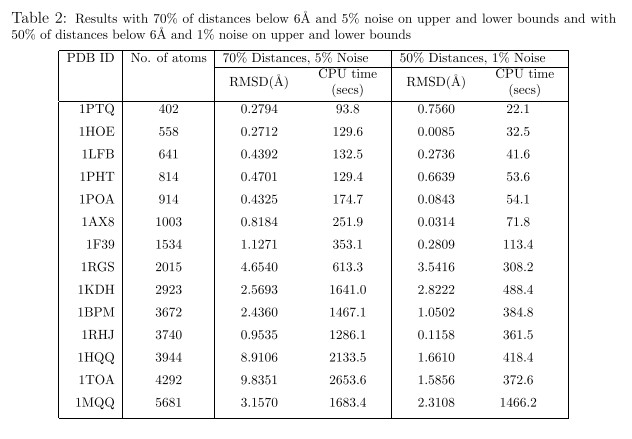
\includegraphics[width=\textwidth]{BiswasYe.jpg}
  \caption{Results in [Biswas-Toh-Ye 2007]}
\end{figure}
}

\frame{
\begin{figure}
  \centering
  \subfigure{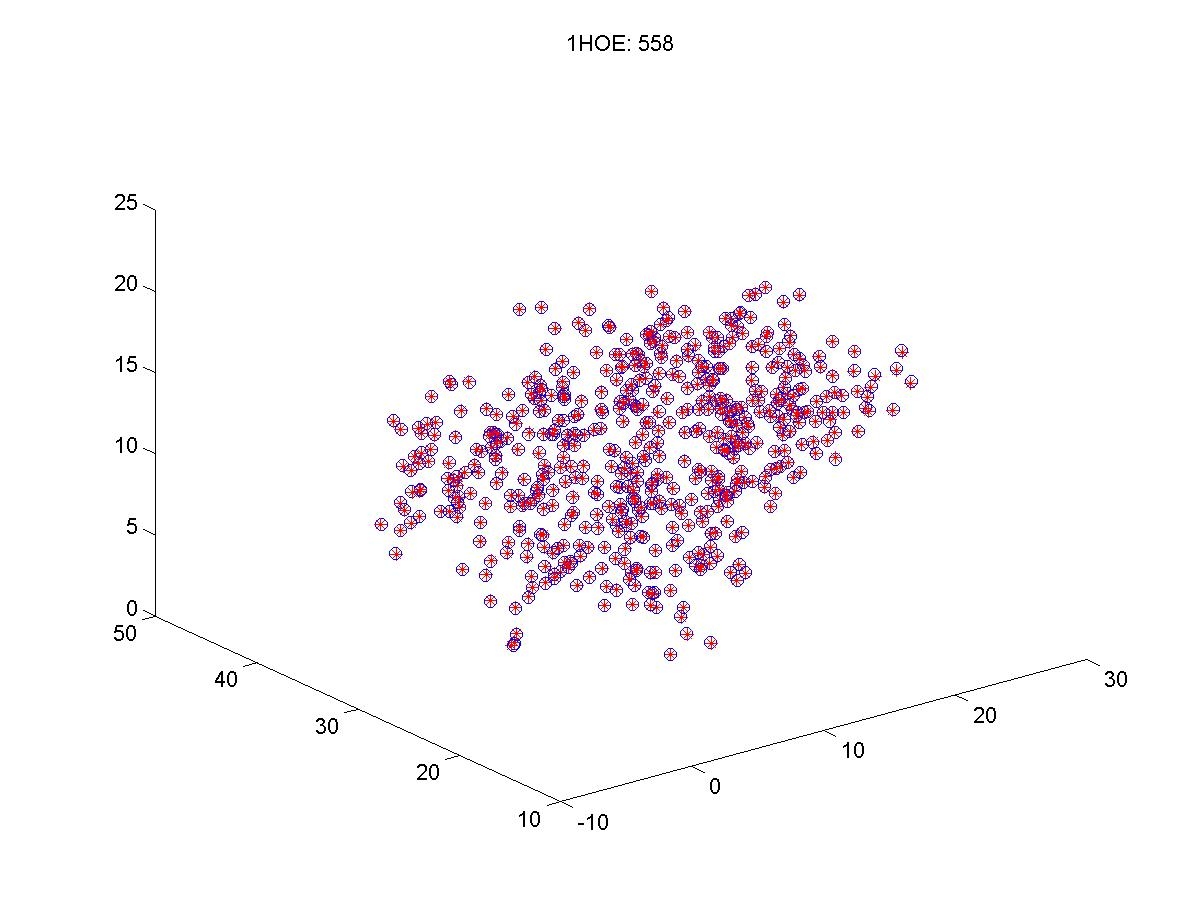
\includegraphics[width=0.45\textwidth]{1HOE51.jpg}}
  \subfigure{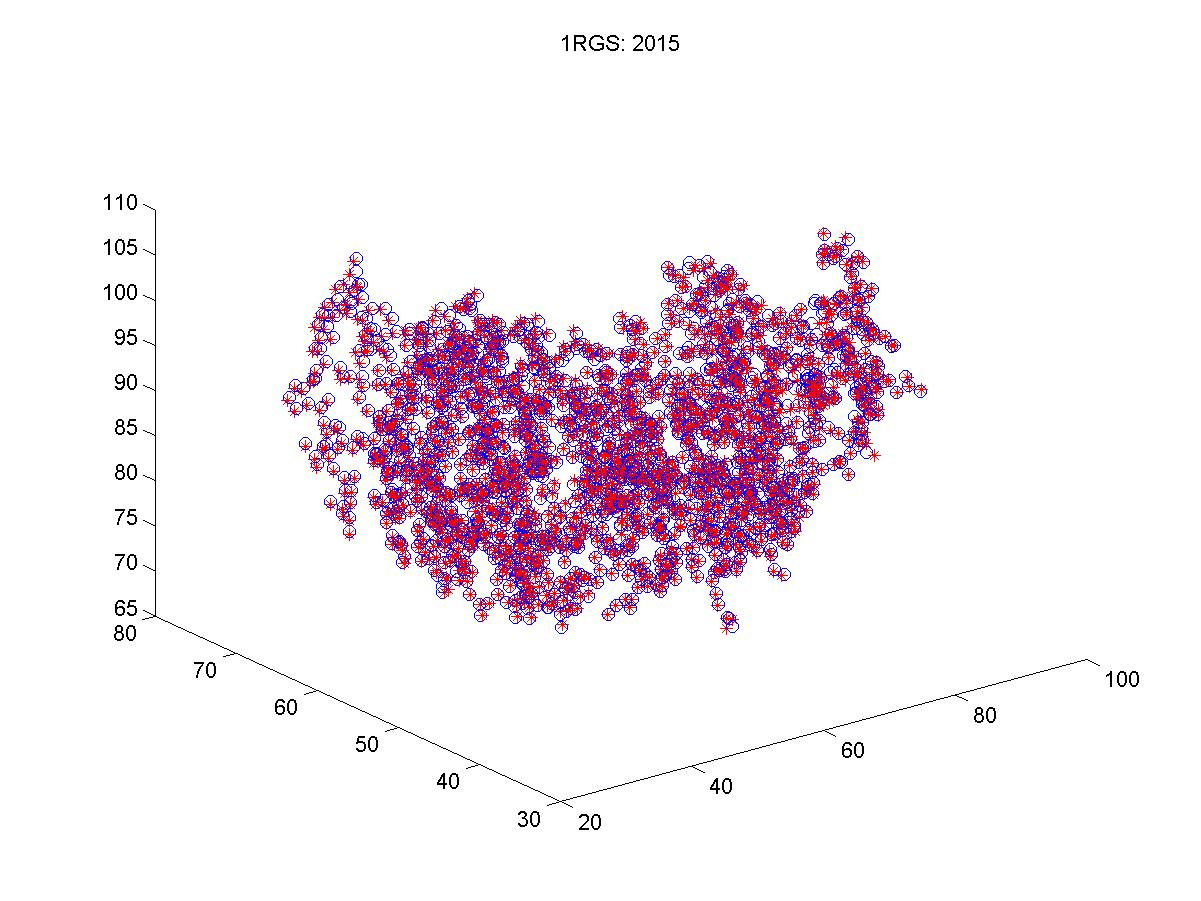
\includegraphics[width=0.45\textwidth]{1RGS51.jpg}}
  \subfigure{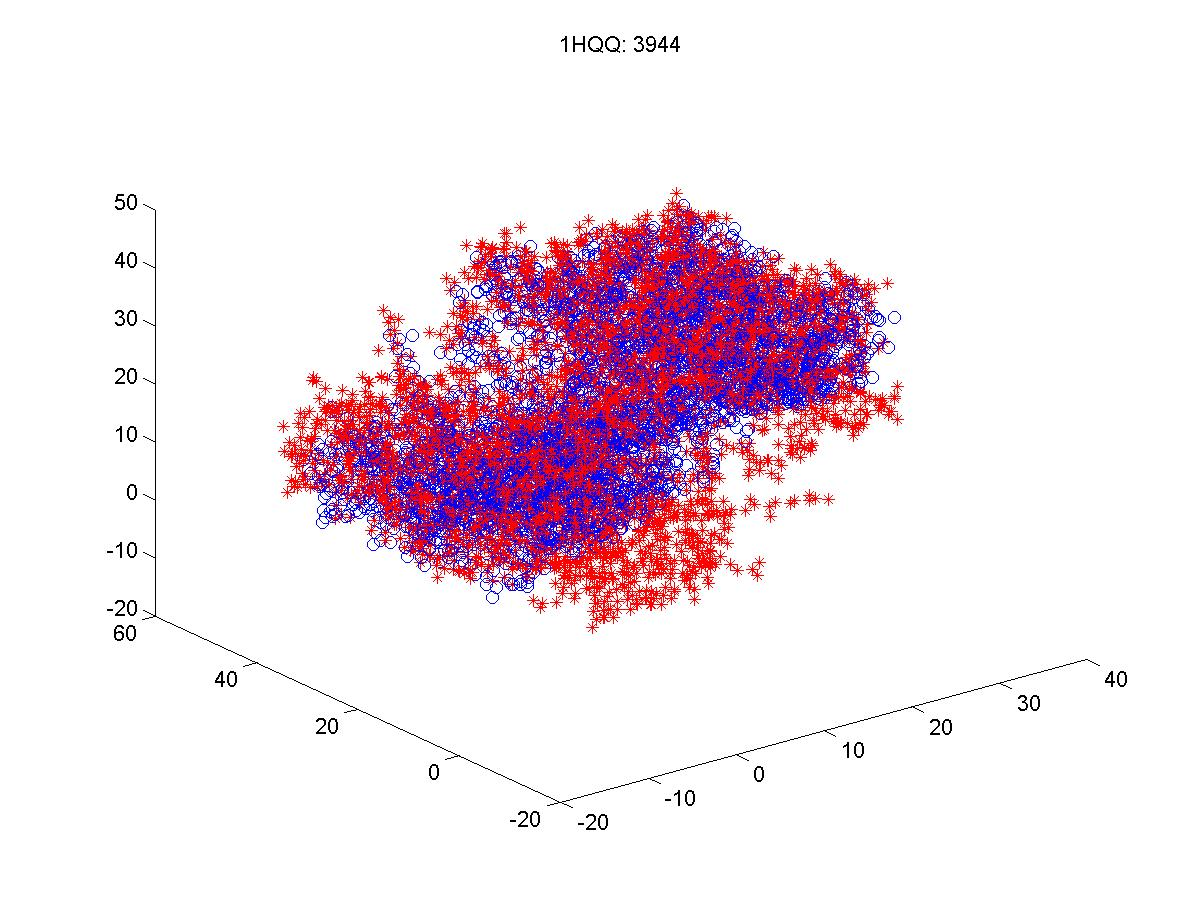
\includegraphics[width=0.45\textwidth]{1HQQ51.jpg}}
  \subfigure{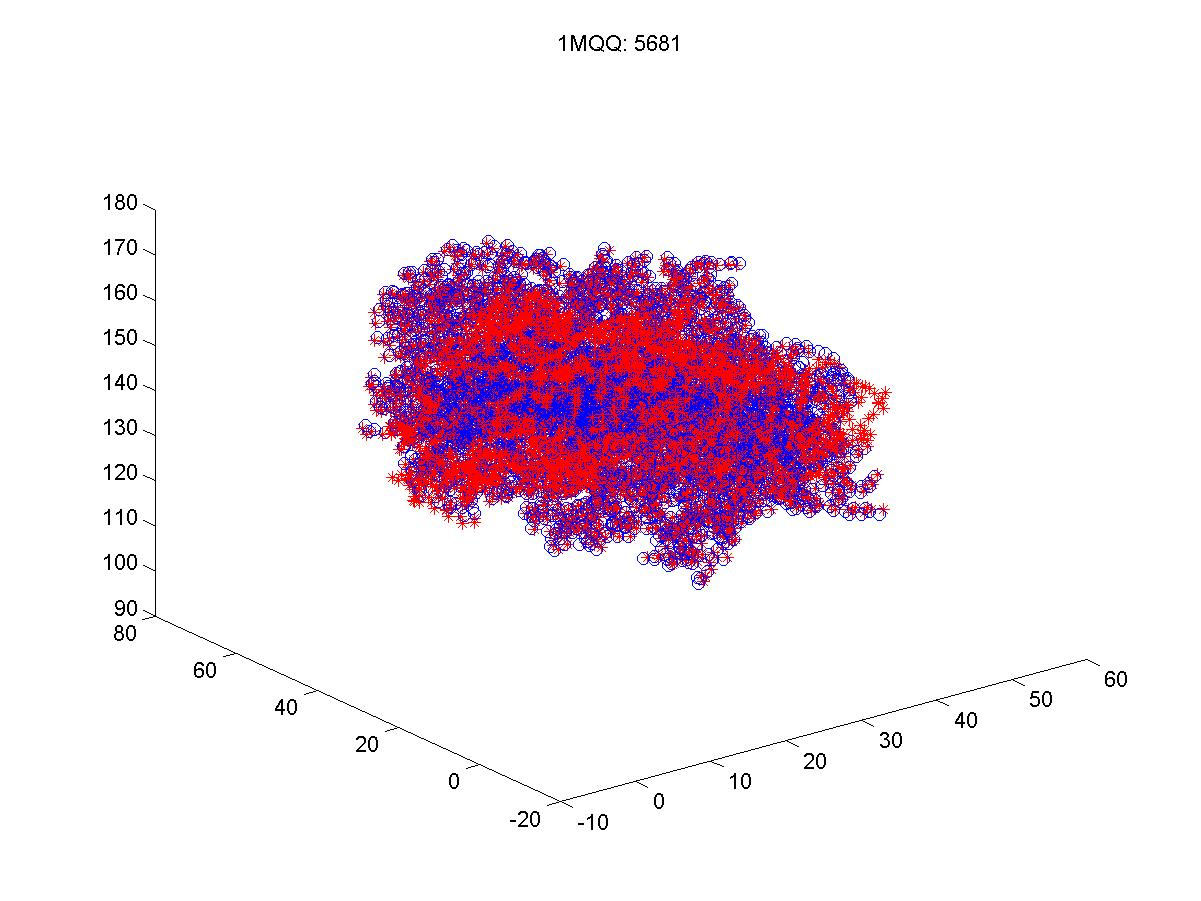
\includegraphics[width=0.45\textwidth]{1MQQ51.jpg}}
  \caption{cutoff={\red 5}{\AA}, noise={\red 0.01}}
\end{figure}
}

\frame{
\begin{figure}
  \centering
  \subfigure{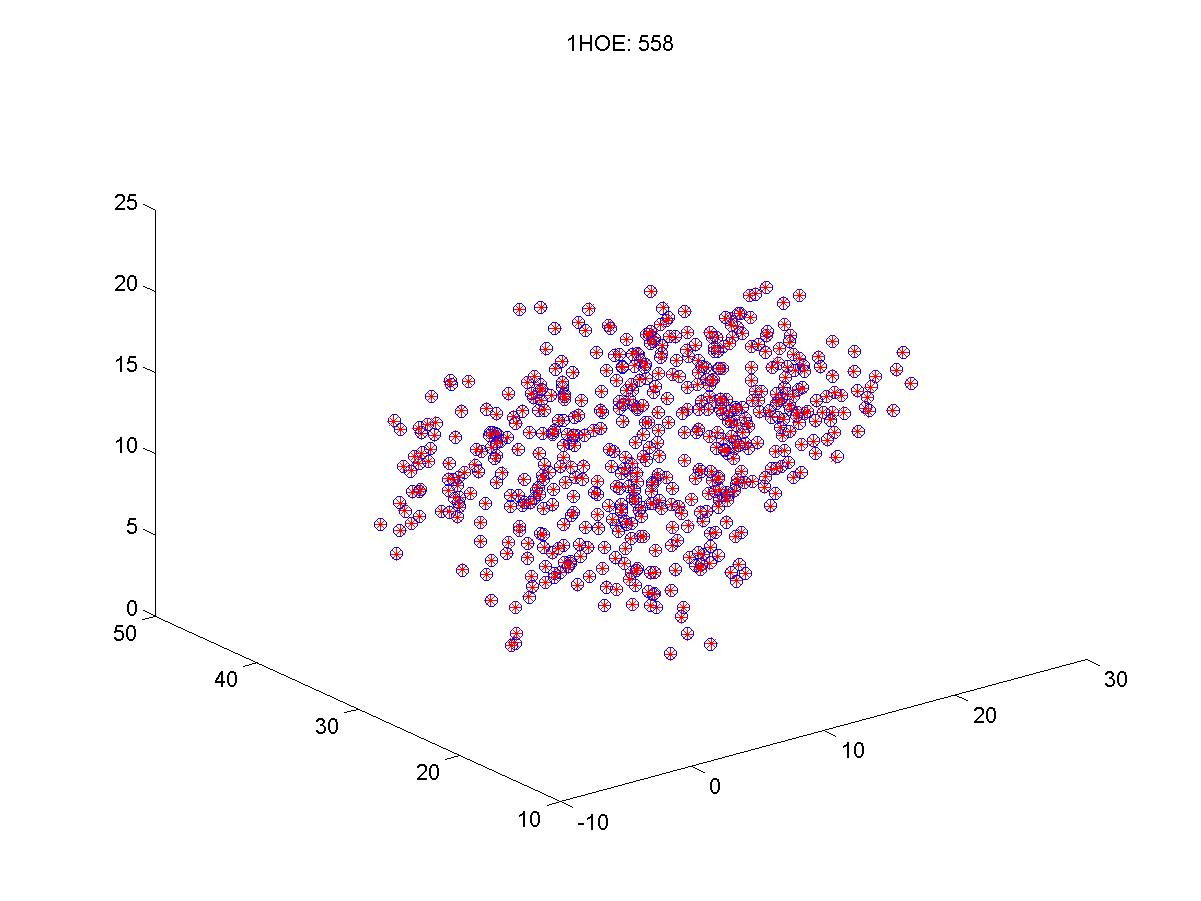
\includegraphics[width=0.45\textwidth]{1HOE61.jpg}}
  \subfigure{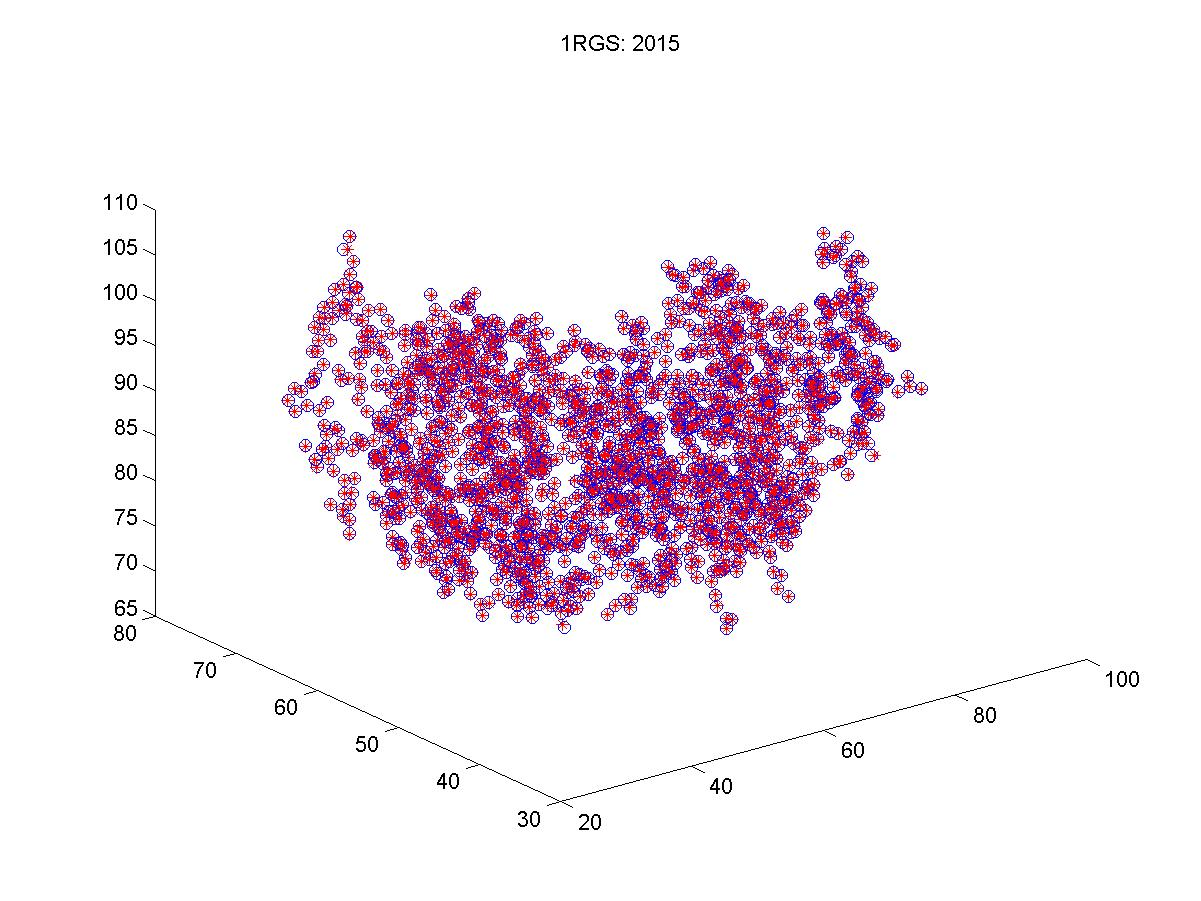
\includegraphics[width=0.45\textwidth]{1RGS61.jpg}}
  \subfigure{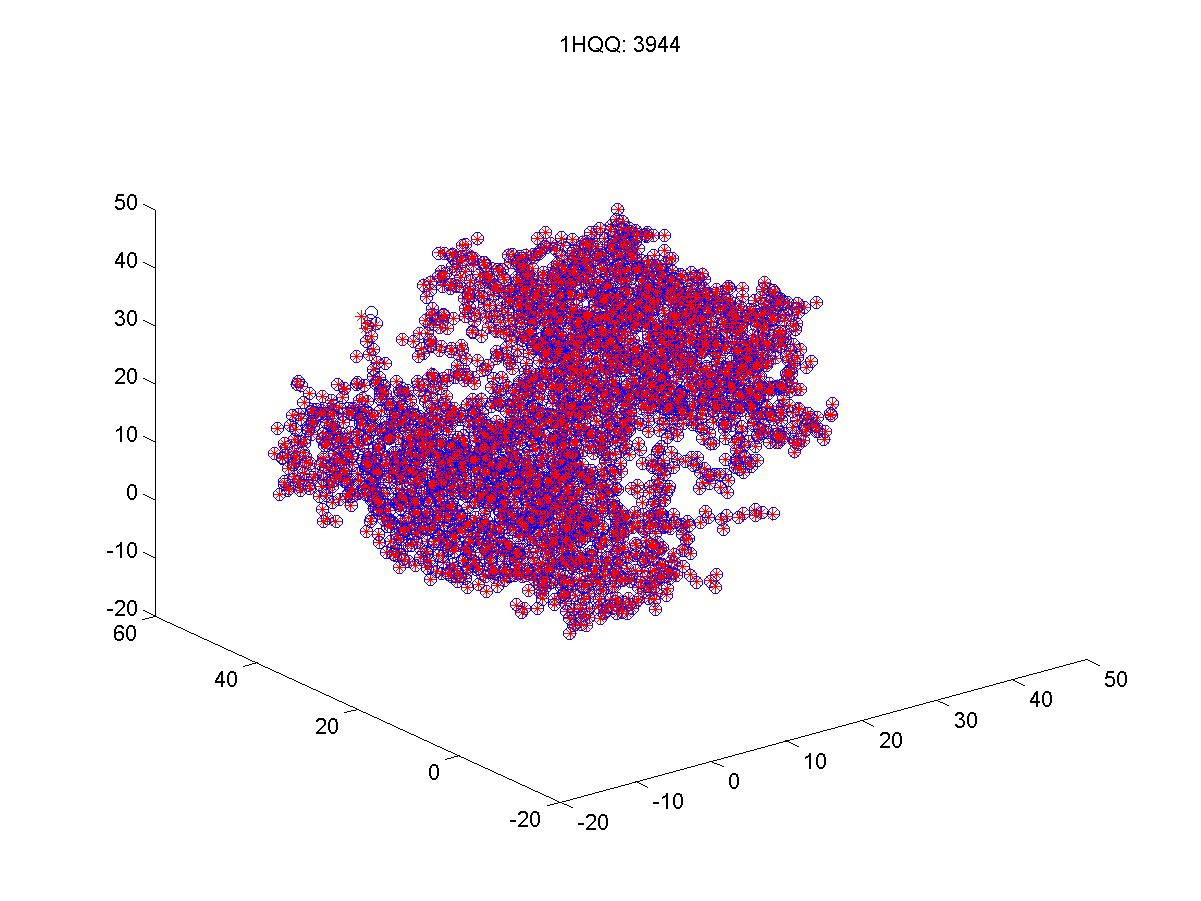
\includegraphics[width=0.45\textwidth]{1HQQ61.jpg}}
  \subfigure{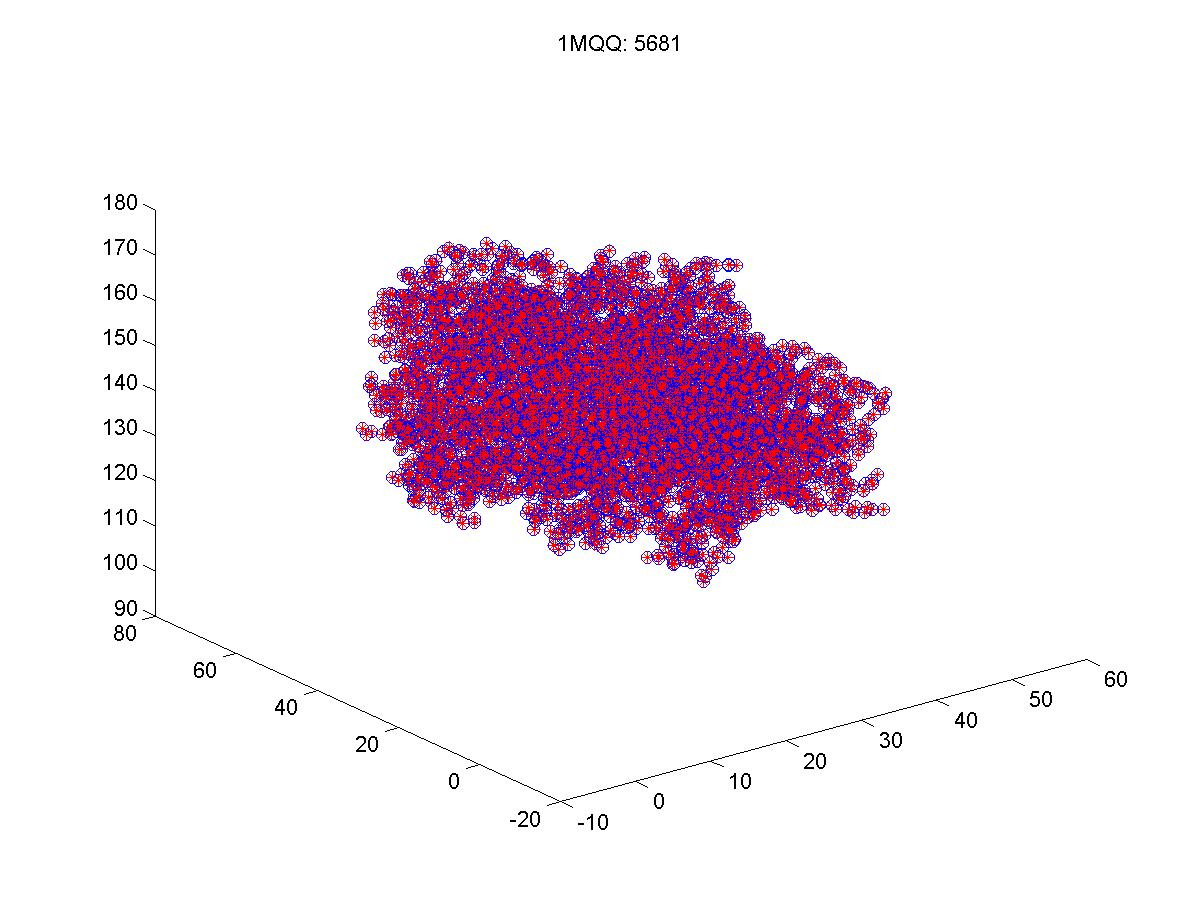
\includegraphics[width=0.45\textwidth]{1MQQ61.jpg}}
  \caption{cutoff={\red 6}{\AA}, noise={\red 0.01}}
\end{figure}
}

\frame{
\begin{figure}
  \centering
  \subfigure{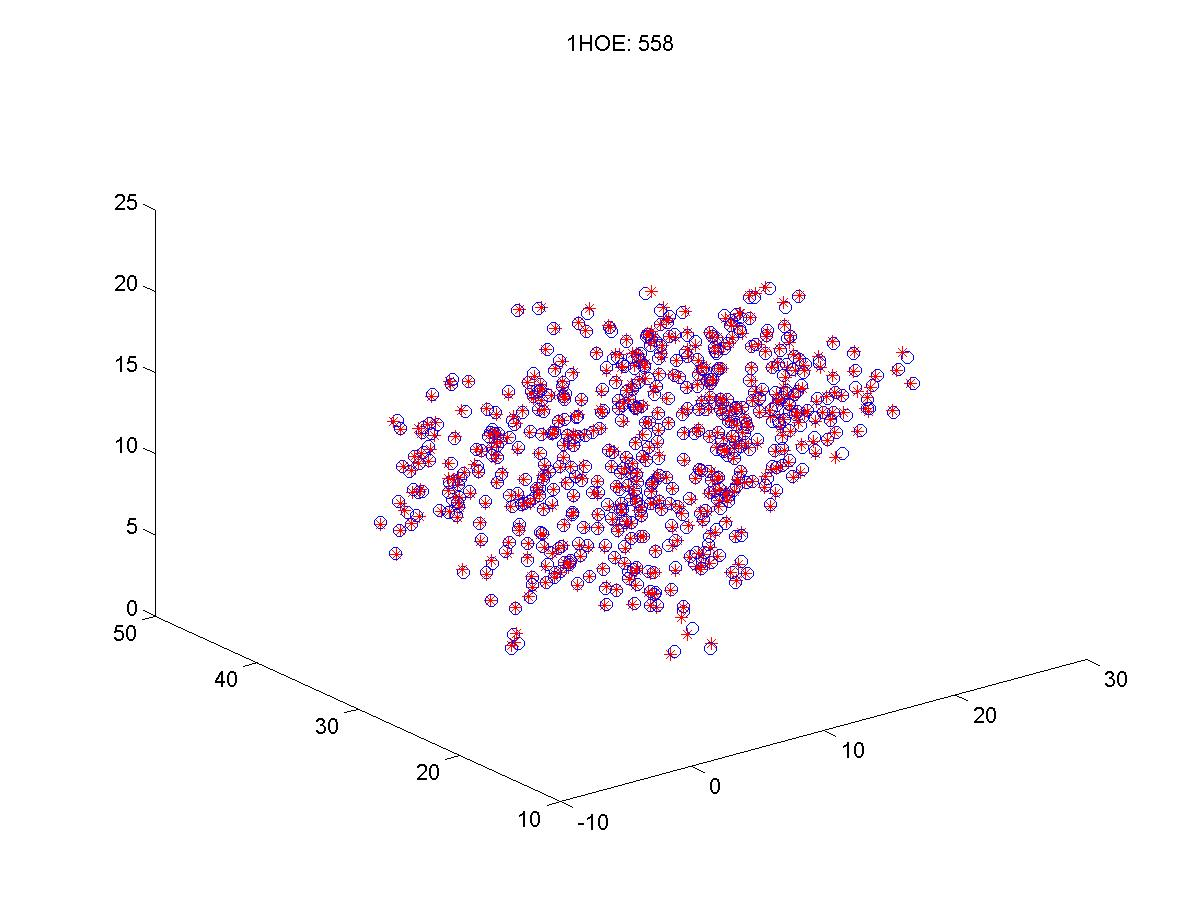
\includegraphics[width=0.45\textwidth]{1HOE65.jpg}}
  \subfigure{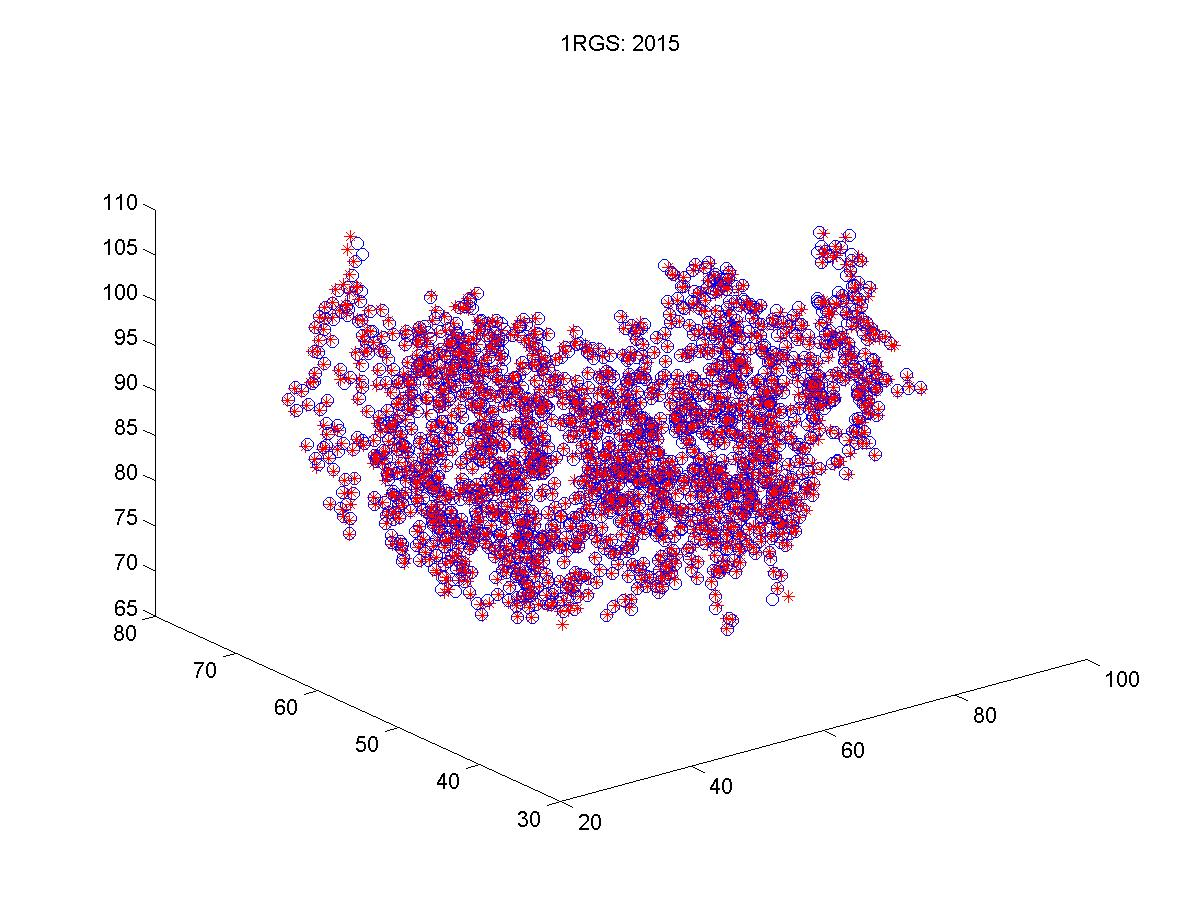
\includegraphics[width=0.45\textwidth]{1RGS65.jpg}}
  \subfigure{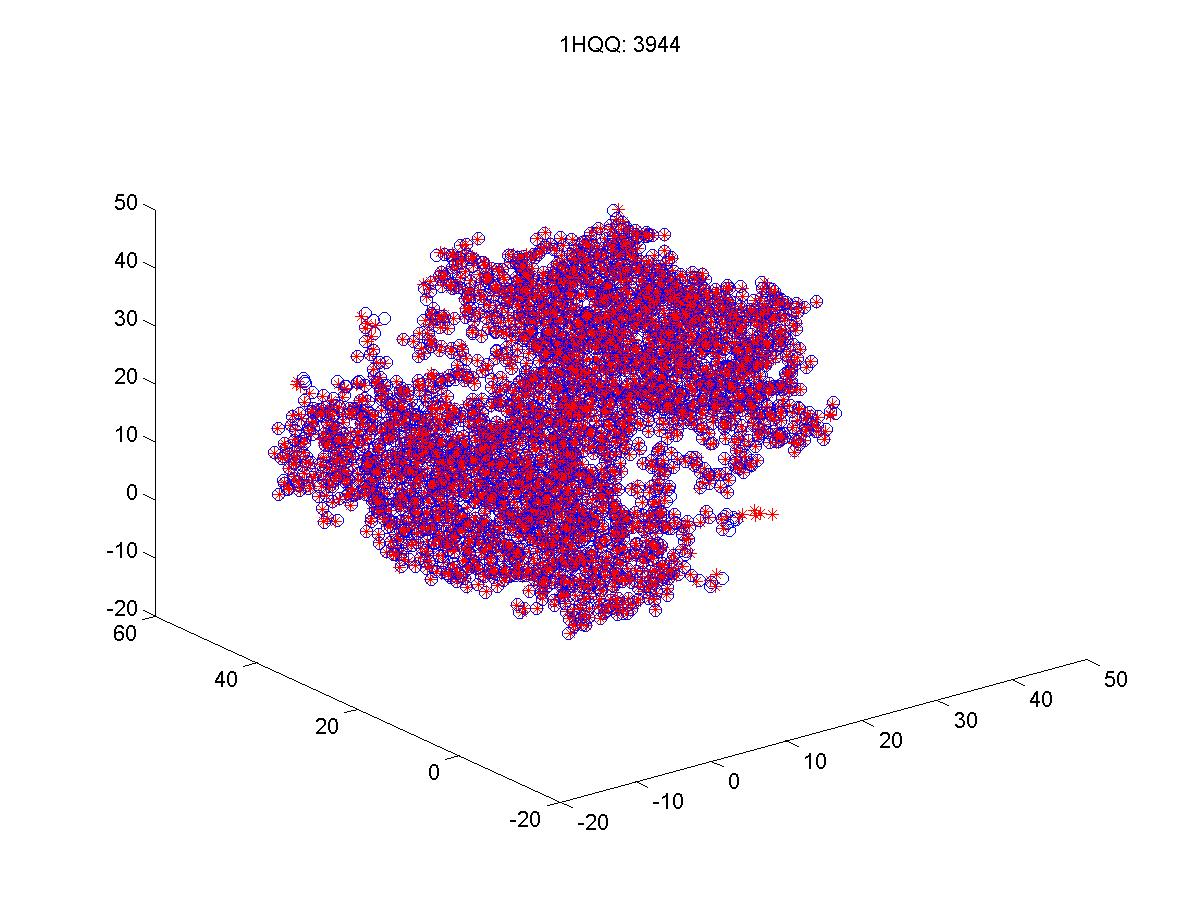
\includegraphics[width=0.45\textwidth]{1HQQ65.jpg}}
  \subfigure{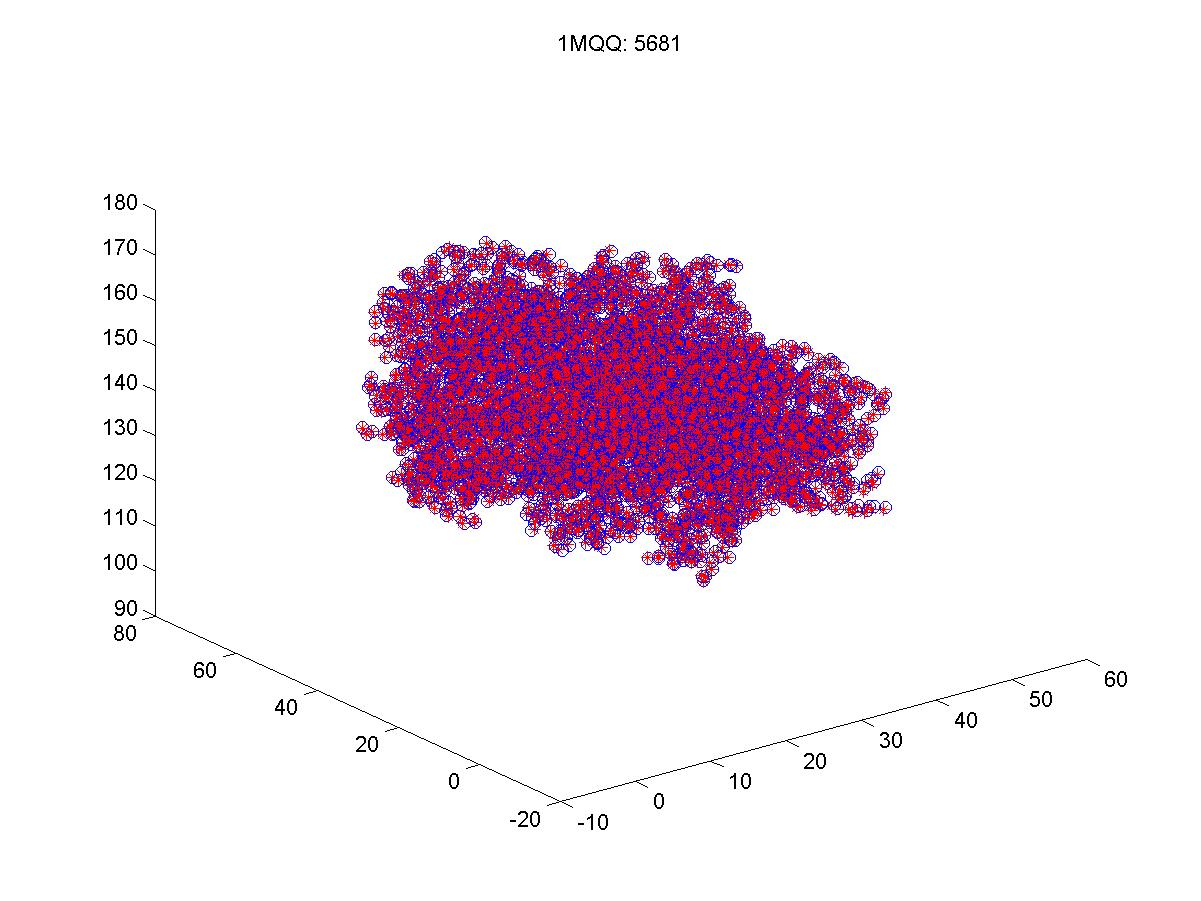
\includegraphics[width=0.45\textwidth]{1MQQ65.jpg}}
  \caption{cutoff={\red 6}{\AA}, noise={\red 0.05}}
\end{figure}
}

\frame{
\begin{figure}
  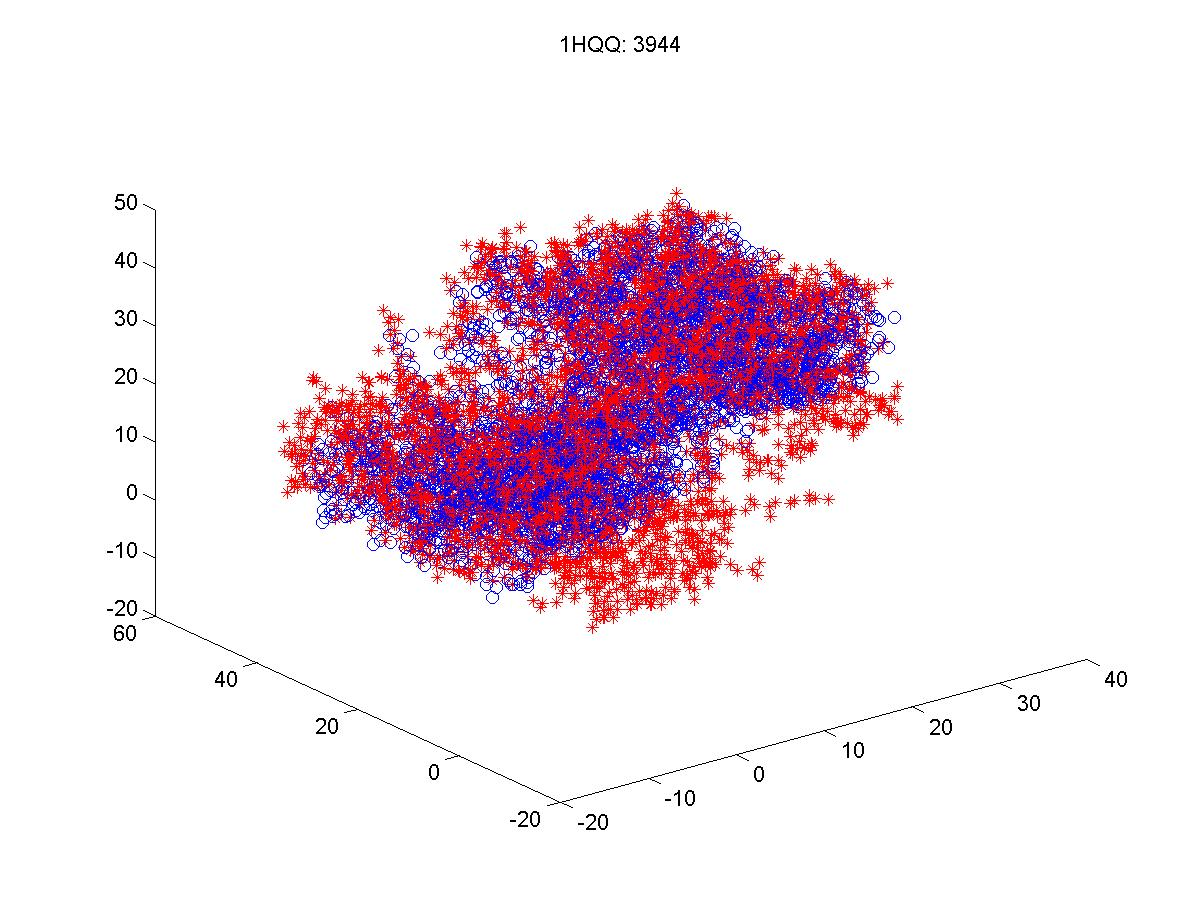
\includegraphics[width=\textwidth]{1HQQ51.jpg}
\end{figure}
}

\frame{
\begin{figure}
  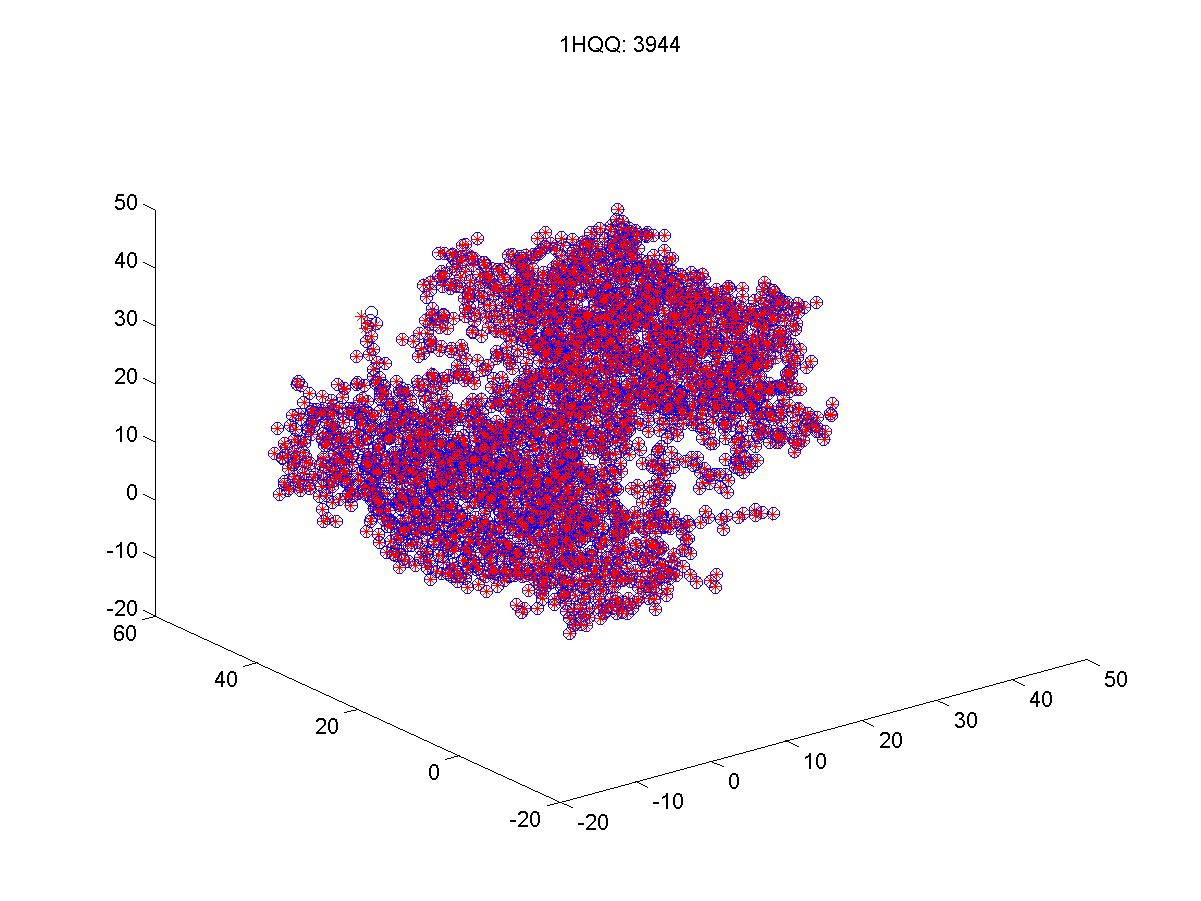
\includegraphics[width=\textwidth]{1HQQ61.jpg}
\end{figure}
}

\frame{
\begin{figure}
  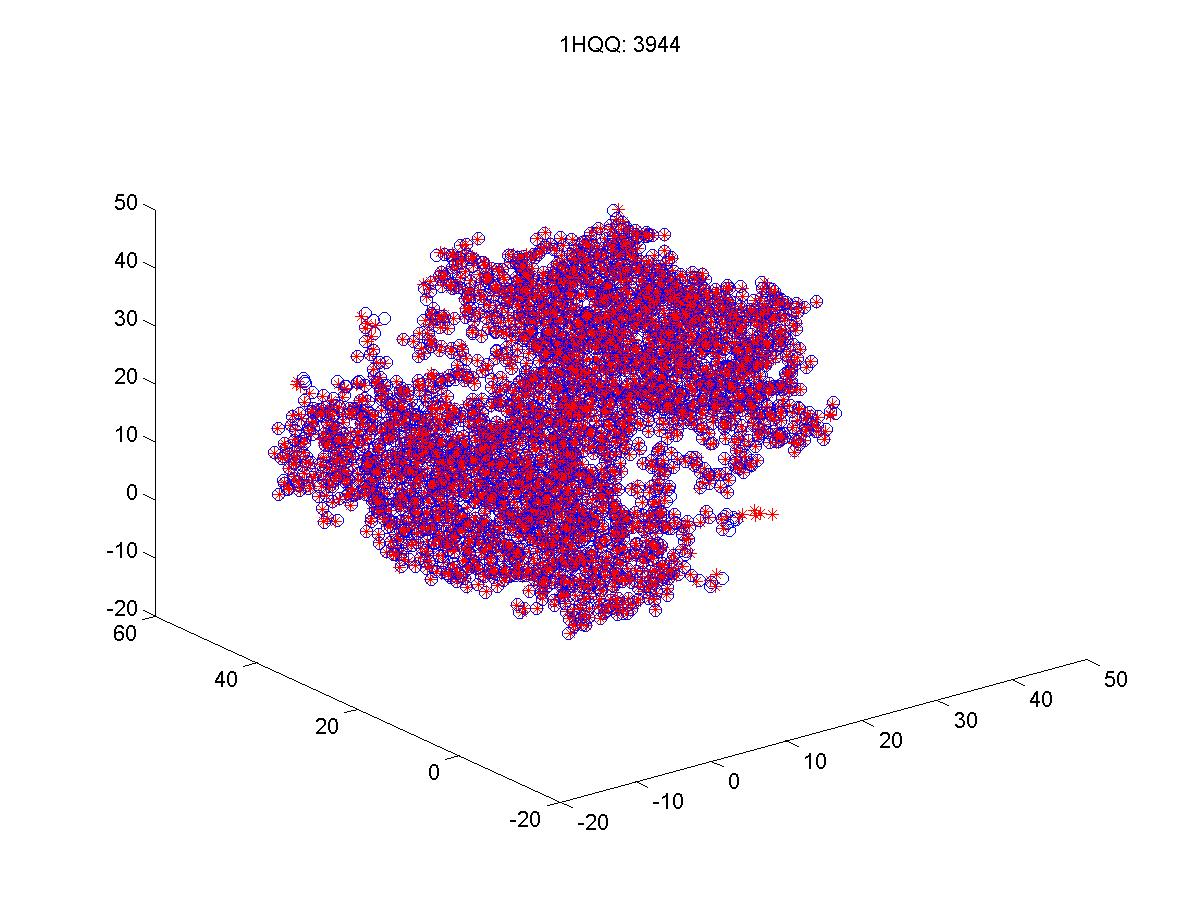
\includegraphics[width=\textwidth]{1HQQ65.jpg}
\end{figure}
}

\section{Ongoing works}
\frame{
\frametitle{Ongoing works}
\begin{itemize}
  \item Further study the properties of error function, then design a fast algorithm.
  \item Extend our algorithm to solve distance geometry problem with distance bounds.
  \item Produce an animation to see how these points were built up one by one.
\end{itemize}
}



%\frame{
%\frametitle{Application \Rmnum{1}: Graph Realization}
%\begin{figure}
%  \centering
%  \subfigure{ 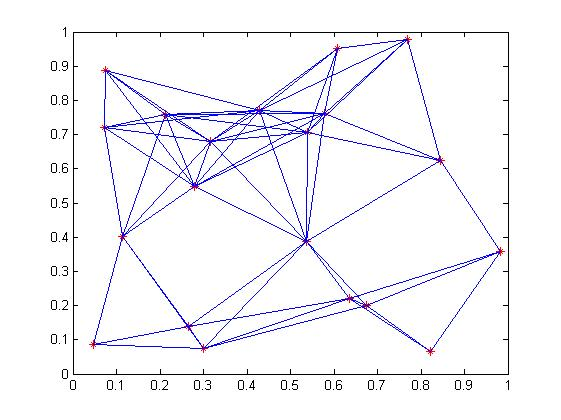
\includegraphics[width=5cm]{GraphRealization.jpg} }
%  \subfigure{ 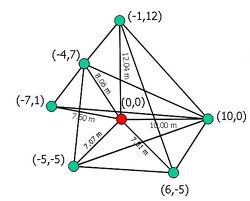
\includegraphics[width=5cm]{GraphRealization2.jpg} }
%  \caption{ Graph Realization in 2D}
%\end{figure}
%\begin{center}
%  Given a graph G=(V,E), each edge has a weight.
%\end{center}
%}
%
%\frame{
%\frametitle{Application \Rmnum{2}: Protein Structure Determination}
%\begin{figure}[htp]
%    \centering
%    \subfigure{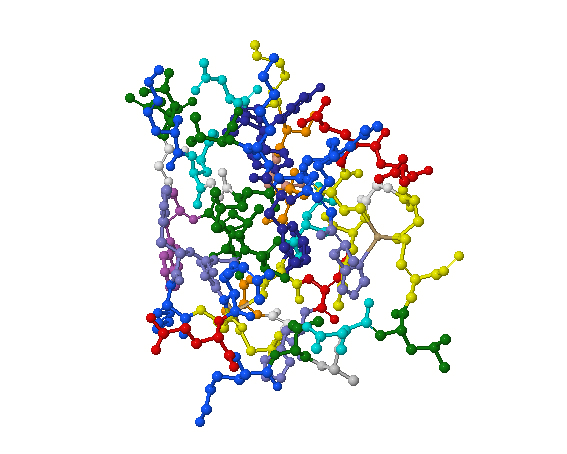
\includegraphics[width=5cm]{1PTQ2.jpg} }
%    \subfigure{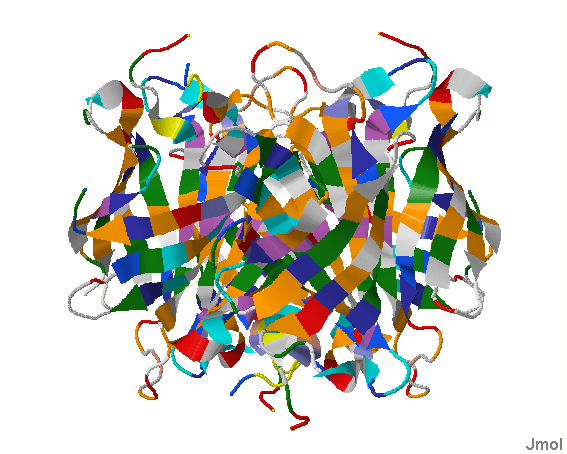
\includegraphics[width=5cm]{1HQQ2.jpg} }
%    \caption{Two proteins: 1PTQ and 1HQQ, in different display ways}
%\end{figure}
%\begin{center}
%  Measure distances: NMR, X ray crystallography.
%\end{center}
%}
%
%\frame{
%\frametitle{Application \Rmnum{3}: Sensor Network Localization}
%\begin{figure}[htp]
%    \centering
%    \subfigure{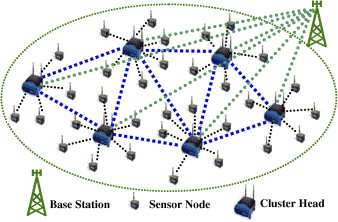
\includegraphics[width=4.5cm]{sensor2.jpg} }
%    \subfigure{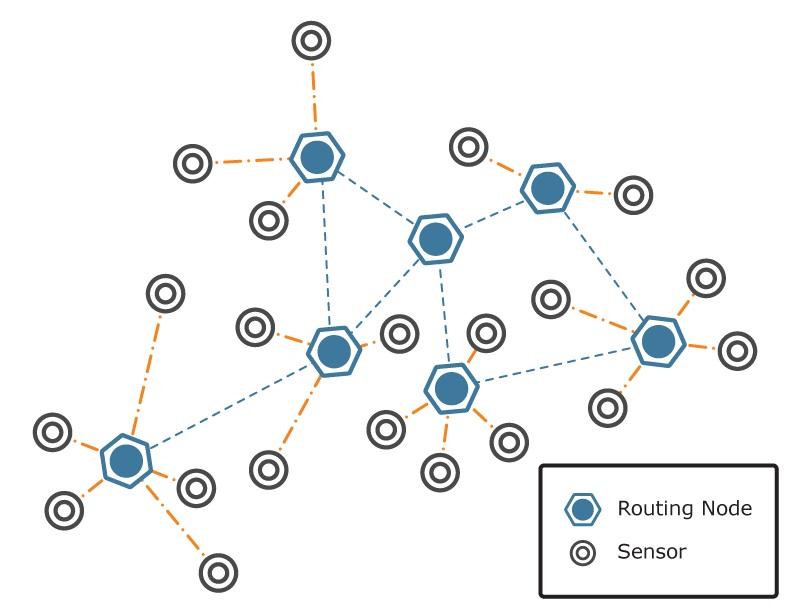
\includegraphics[width=4.5cm]{sensor1.jpg} }
%    \caption{Illustration of wireless sensor networks}
%\end{figure}
%}
%
%\section{Related works}
%\frame{
%\frametitle{Related works}
%\begin{itemize}%[$\blacktriangleright$]
%  \item Matrix Decomposition Method (Blumenthal-1953, Torgerson-1958)
%  \item The Embedding Algorithm (Crippen-Havel-1988)
%  \item Global Smoothing Algorithm (Mor\'{e}-Wu-1997)
%  \item Geometric Buildup Method (Dong-Wu-2002, Sit-Wu-Yuan-2009)
%  \item SDP Relaxation Method (Biswas-Toh-Ye-2007)
%  \item ...
%\end{itemize}
%}
%
%\frame{
%\frametitle{Matrix Decomposition Method}
%{\red DG problem with full set of exact distances} \\
%%\textrm{}\\
%\small{
%Given a full set of distances, $d_{i,j} = \| x_{i}-x_{j} \|, \quad i,j=1,2,\ldots,n.$ \\
%\begin{itemize}%[$\blacktriangleright$]
%  \item Set $x_{n} = (0,0,0\Tran)$, we have
%      \begin{eqnarray}
%      % \nonumber to remove numbering (before each equation)
%        \nonumber d_{i,j}^{2} &=& \|x_{i}-x_{j}\|^{2} \\
%        \nonumber             &=& \|x_{i}\|^{2}-2\Tran x_{i} x_{j}+\|x_{j}\|^{2} \\
%                              &=& d_{i,n}^{2}-2\Tran x_{i} x_{j}+d_{j,n}^{2}, \qquad  i,j=1,2,\ldots,n-1 \label{eq1}
%      \end{eqnarray} \\
%      \vspace{0.3cm}
%  \item Define $ X=(x_{1},x_{2},\ldots,x_{n}\Tran)$ and $D=\{(d_{i,n}^{2}-d_{i,j}^{2}+d_{j,n}^{2})/2: i,j=1,2,\ldots,n-1\}$,  (\ref{eq1}) $\Rightarrow {\red X\Tran X=D}$.\\
%      \vspace{0.3cm}
%  \item Let $D=U\Sigma\Tran U$, $V=U(:,1:3)$ and $\Lambda=\Sigma(1:3,1:3)$. Then $X = V\Lambda^{1/2}$ solves the problem. [{\blue Eckart and Young 1936}]
%\end{itemize} }
%}
%
%\frame{
%\frametitle{Unconstrained optimization: Error functions}
%\begin{itemize}
%  \item stress function
%        \begin{equation*}
%          Stress(x_{1},x_{2},\ldots,x_{n}) = \sum_{(i,j)\in S} (\|x_{i}-x_{j}\|-d_{i,j})^{2},
%        \end{equation*}
%  \item smoothed stress function
%  \begin{equation*}
%          SStress(x_{1},x_{2},\ldots,x_{n}) = \sum_{(i,j)\in S} (\|x_{i}-x_{j}\|^{{\red 2}}-d_{i,j}^{{\red 2}})^{2},
%        \end{equation*}
%  \item generalized stress function
%        \footnotesize{
%        \begin{equation*}
%          GStress(x_{1},x_{2},\ldots,x_{n}) = \sum_{(i,j)\in S} \min\nolimits^{2} \{\frac{\|x_{i}-x_{j}\|^{2}-l_{i,j}^2}{l_{i,j}^{2}},0\} + \max\nolimits^{2} \{\frac{\|x_{i}-x_{j}\|^{2}-u_{i,j}^2}{u_{i,j}^{2}},0\}.
%        \end{equation*} }
%\end{itemize}
%}
%
%\frame{
%\frametitle{Goal and Difficulties}
%\begin{itemize}
%  \item Goal: minimize the chosen error function to the {\red global} minimizer---{\red zero}
%      \vspace{0.3cm}
%  \item Difficulties: NP-hard in general
%  \begin{enumerate}[--]
%    \item too many local minimizers
%    \item possibly nonsmooth
%    \item large-scale problems
%  \end{enumerate}
%\end{itemize}
%}
%
%\section{Our proposed error function and algorithm}
%\frame{
%\frametitle{Our proposed error function}
%\begin{minipage}{0.55\textwidth}
%Define h: $\mathbb{R}_{++}\rightarrow \mathbb{R}$ as below,
%\begin{displaymath}
%  h(x) = \left\{ \begin{array}{ll}
%                  \frac{1}{2}(x-1)^{2}, & x\geq 1, \\
%                  x-(1+ln(x)),          & x<1.
%                \end{array}   \right.
%\end{displaymath}
%\end{minipage}
%\begin{minipage}{0.4\textwidth}
%\begin{figure}
%  \centering
%  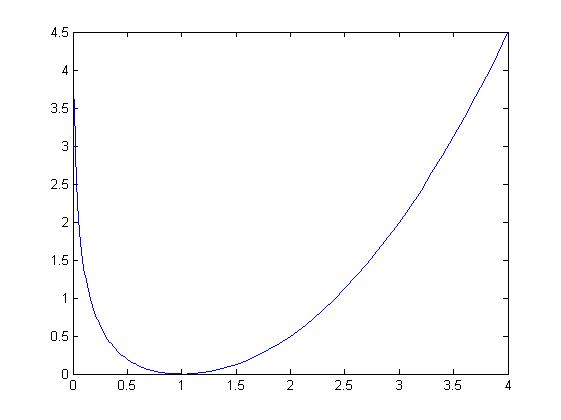
\includegraphics[width=\textwidth]{huke.jpg}
%\end{figure}
%\end{minipage}
%
%\textrm{}\\
%\begin{Thm}
%h(x) is twice continuously differentiable in $(0, +\infty)$, and it achieves its minimum 0 at 1.
%\end{Thm}
%}
%
%\frame{
%\frametitle{But... why this function?}
%\begin{minipage}{0.5\textwidth}
%\begin{figure}
%  \centering
%  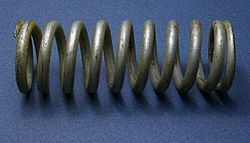
\includegraphics[width=0.8\textwidth]{springs.jpg}\\
%  \caption{ {\orange Hooke's law} models the properties of springs for small changes in length}
%\end{figure}
%\end{minipage}
%\begin{minipage}{0.45\textwidth}
%Force function:
%$$F=\left\{  \begin{array}{ll}
%                  x-1, & x\geq 1, \\
%                  1-\frac{1}{x}, & x<1.
%                \end{array}  \right. $$
%then the energy function is h(x).
%\end{minipage}
%\begin{minipage}{0.5\textwidth}
%Another proposal: \\$h(x)=x-(1+ln(x))$
%\end{minipage}
%\begin{minipage}{0.45\textwidth}
%\begin{figure}
%  \centering
%  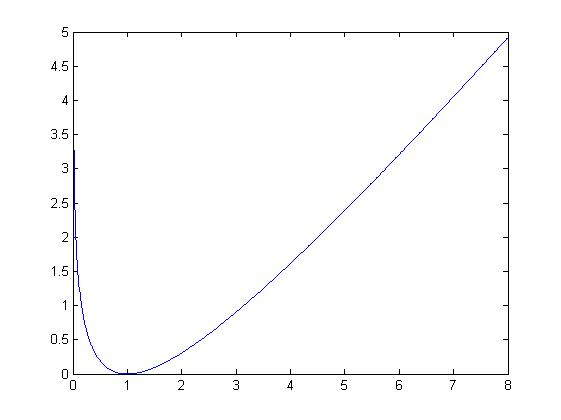
\includegraphics[width=\textwidth]{error2.jpg}\\
%\end{figure}
%\end{minipage}
%}
%
%
%\frame{
%\frametitle{Modeling and Solution idea}
%Using our error function, the distance geometry problem can be formulated as
%{\red
%\begin{equation}
%  \min \quad f(x_{1},x_{2},\ldots,x_{n})=\sum_{(i,j)\in S} h(\frac{\|x_{i}-x_{j}\|}{d_{i,j}}).
%\end{equation} }
%\vspace{0.3cm}
%\begin{itemize}
%  \item Observation:
%  \begin{enumerate}[--]
%    \item huge items in the objective function
%    \item variables are mixed together $\Rightarrow$ not easy to calculate Hessian matrix
%  \end{enumerate}
%  \item Solution idea:
%  \begin{enumerate}[--]
%    \item use first-order algorithm --- "alternative direction method" to solve it\\
%    $\Rightarrow$ fixed the others, adjust $x_{i}(i=1,\ldots,n)$ in turn.
%  \end{enumerate}
%\end{itemize}
%}
%
%
%\frame{
%\frametitle{Trust region subproblem}
%Let $\overline{f}(x)=\sum_{j\in N(i)} h(\frac{\|x-x_{j}\|}{d_{i,j}})$, where $N(i)$ is the neighbourhood of point $i$, then the "trust region subproblem" at each iteration is as following,
%\begin{equation}\label{tr}
%  \begin{array}{ccl}
%  \min\limits_{s} & \Tran{s}\nabla\overline{f}(x_{i}) + \frac{1}{2}\Tran{s}\nabla^{2}\overline{f}(x_{i})s & \triangleq q(x) \\
%  \st      & \|s\| \leq \Delta. & \\
%  \end{array}
%\end{equation}
%\begin{figure}
%  \centering
%  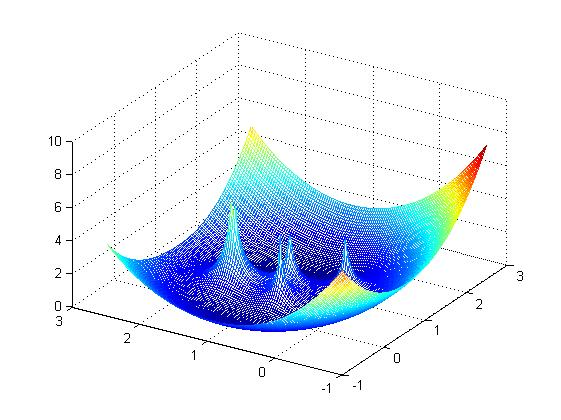
\includegraphics[width=0.5\textwidth]{energy.jpg}\\
%  %\caption{Illustration of $\overline{f}(x)$}
%\end{figure}
%}
%
%\frame{
%\frametitle{Trust region subproblem (Cont'd)}
%\footnotesize{
%\begin{Thm}
%Define $\overline{h}: \Real^{d}\rightarrow \Real, \overline{h}(x)=h(\frac{\|x-a\|}{d})$, where $a\in \Real^{d}$ and $d\in \Real$ are constants, then
%\begin{itemize}
%  \item $$ \nabla \overline{h}(y)=\frac{y}{d\|y\|}-\frac{y}{\|y\|^{2}},$$
%  and
%$$ \nabla^{2} \overline{h}(y)=-\frac{y\Tran{y}}{d\|y\|^{3}} + \frac{2y\Tran{y}}{\|y\|^{4}} + (\frac{1}{d\|y\|}-\frac{1}{\|y\|^{2}})I$$
%$$\qquad \quad=(\frac{1}{d\|y\|}-\frac{1}{\|y\|^{2}})(I-\frac{y\Tran{y}}{\|y\|^{2}}) + \frac{y\Tran{y}}{\|y\|^{4}},$$
%where
%$$y=x-a \textrm{ and I is the identity matrix}.$$
%  \item if $\|y\| \geq d, \nabla^{2} \overline{h} (y)$ is positive definite, otherwise it can be negative definite.
%\end{itemize}
%\end{Thm} }
%}
%
%\frame{
%\frametitle{Stopping criteria}
%\begin{enumerate}
%  \item the objective function or the improvement is small enough, i.e.
%  $$f_{k}< tol~~~or~~~|f_{k}-f_{k-1}|< tol$$
%  \item the norm of the gradient is small enough, i.e.
%  $$\|\nabla f(x)\|< MinNorm$$
%  where $tol,~MinNorm$ are some given small numbers, for instance, $10^{-5}$.
%  \item the outer iteration achieves its maximum permitted number, i.e. $k<MaxItr$
%\end{enumerate}
%\vspace{0.5cm}
%\begin{enumerate}[{\color{black} $\spadesuit$ }]
%  \item One of the above three criteria is satisfied, the algorithm will stop.
%\end{enumerate}
%}
%
%\frame{
%\frametitle{Algorithm framework \Rmnum{1}}
%\begin{algorithm}[H]
%\SetKwInOut{Init}{Initialization}
%\vspace{0.3cm}
%\Init{Give initial points and set some parameters}
%\While{stopping criteria not satisfied}{
%\For{i=1:n}{ Solve trust region subproblem (\ref{tr}) to obtain $s_{i}$, let
%$$r_{i} = \frac{\overline{f}(x_{i})-\overline{f}(x_{i}+s_{i})}{q(x_{i})-q(x_{i}+s_{i})}$$
%According to $r_{i}$ to determine to accept $s_{i}$ or not, and adjust $\Delta_{i}$\;
%}
%}
%\caption{Trust Region Error Minimization Method}
%\label{algtr}
%\end{algorithm}
%}
%
%\frame{
%\frametitle{Nonmonotone Newton step}
%\begin{itemize}
%  \item Let $\overline{f}(x)$ be defined as before, then "Newton step" can be given as below,
%      $$d_{i}^{N} = -(\nabla^{2}\overline{f}(x_{i}))^{-1}\nabla\overline{f}(x_{i})$$
%      Let search direction be
%      \begin{equation}\label{Ndirection}
%      d_{i} = \left\{
%      \begin{array}{ll}
%      d_{i}^{N} & if~\nabla^{2}\overline{f}(x_{i})~is~positive~definite,\\ -\nabla\overline{f}(x_{i}) & otherwise,
%      \end{array} \right.
%      \end{equation}
%      which is a descent direction.
%  \item Search for stepsize $\alpha_{i}$ by backtracking (start at 1), such that
%      \begin{equation}\label{Nstepsize}
%      f(x_{i}+\alpha_{i}d_{i},x_{-i})< MaxF + \frac{1}{2}\alpha_{i}\Tran{d_{i}}\nabla\overline{f}(x_{i})%\max_{k=1:M} {fval(i-k)}
%      \end{equation}
%      where $MaxF$ is the maximum objective function value of lastest M step.
%\end{itemize}
%}
%
%\frame{
%\frametitle{Algorithm framework \Rmnum{2}}
%\begin{algorithm}[H]
%\SetKwInOut{Init}{Initialization}
%\vspace{0.3cm}
%\Init{Give initial points and set some parameters}
%\While{stopping criteria not satisfied}{
%\For{i=1:n}{
%Calculate search direction $d_{i}$ by (\ref{Ndirection})\;
%Calculate stepsize $\alpha_{i}$ by (\ref{Nstepsize})\;
%Set $x_{i}\leftarrow x_{i}+\alpha_{i}d_{i}$
%}
%}
%\caption{Nonmonotone Newton Error Minimization Method}
%\label{algNewton}
%\end{algorithm}
%}
%
%\frame{
%\frametitle{Algorithm framework \Rmnum{3}}
%\begin{algorithm}[H]
%\vspace{0.4cm}
%\begin{enumerate}
%  \item Apply \textbf{Algorithm \ref{algtr}} for K iterations,
%  \item Apply \textbf{Algorithm \ref{algNewton}} then.
%\end{enumerate}
%\caption{Trust Region-Newton Error Minimization Method}
%\end{algorithm}
%
%\vspace{1cm}
%K can be set adaptively.
%}
%
%\section{Numerical experiments}
%%\frame{
%%\frametitle{Problem and parameters}
%%\begin{itemize}
%%  \item Download structure data from Protein Data Bank(PDB), obtain the original coordinates X.
%%  \item Use \emph{{\blue disk graph model}} to construct distance matrix, usually set cutoff as 5{\AA} or 6{\AA}.
%%  \item Solve the problem with our algorithm to get Computed coordinates Y, then compare it with X, using the criteria defined as below,
%%        $$ RMSD(X,Y) = \min_{Q,T}\|X-YQ-T\|_{F}/\sqrt{n} $$
%%\end{itemize}
%%}
%
%\frame{
%\frametitle{Experiments construction}
%\begin{itemize}
%  \item Uniformly sample nodes in square [0,1]x[0,1].
%  \item Generate distance matrix by \emph{{\orange disk graph model}}, usually set cutoff=0.2, thus about 10\% distance are available.
%  \item Generate initial points with 20\% perturbation, more specifically,
%      $$X0 = X .* (1 + 0.2*(rand(n,2)-0.5)).$$
%  \item Use function value and cost time as the compare criteria.
%\end{itemize}
%}
%
%\frame{
%\frametitle{Monotone VS Nonmonotone stepsize}
%\centering
%\begin{tabular}{|r|c|c|c||r|c|c|c|}
%  \hline
%  \multicolumn{8}{|c|}{$cotoff=0.2, exact~distance, perturbation=20\%, MaxItr=100$} \\
%  \hline
%  \multicolumn{4}{|c||}{$n=100, tol=10^{-3}$} & \multicolumn{4}{c|}{$n=200, tol=10^{-3}$} \\
%  \hline
%  M & iter & fval & t(s) & M & iter & fval & t(s)\\
%  \hline
%    1 & 17 & 0.080 & 3.37 &   1 & 100 & 5.206 & 40.40 \\
%    5 & 35 & 0.012 & 3.98 &   5 & 100 & 4.170 & 34.17 \\
%   20 & 32 & 0.014 & 3.86 &  20 & 100 & 1.893 & 34.36 \\
%   50 & 35 & 0.012 & 4.00 &  50 & 100 & 0.263 & 32.44 \\
%  100 & 30 & 0.013 & 3.76 & 100 & 100 & {\blue 0.112} & 31.63\\
%  \hline
%    1 & 36 & 0.474 & 5.30 &   1 &  84 & 0.430 & 31.03 \\
%    5 & 31 & 0.462 & 4.46 &   5 &  65 & 0.417 & 24.25 \\
%   20 & 30 & 0.459 & 4.42 &  20 &  63 & 0.417 & 23.88 \\
%   50 & 28 & 0.456 & 4.33 &  50 &  63 & 0.416 & 23.82 \\
%  100 & 28 & 0.456 & 4.33 & 100 &  63 & 0.415 & 23.81 \\
%  \hline
%\end{tabular} \\
%}
%
%\frame{
%\frametitle{Monotone VS Nonmonotone stepsize}
%\centering
%\begin{tabular}{|r|c|c|c||r|c|c|c|}
%  \hline
%  \multicolumn{8}{|c|}{$cotoff=0.2, exact~distance, perturbation=20\%, MaxItr=100$} \\
%  \hline
%  \multicolumn{4}{|c||}{$n=500, tol=10^{-2}$} & \multicolumn{4}{c|}{$n=1000, tol=10^{-1}$} \\
%  \hline
%  M & iter & fval & t(s) & M & iter & fval & t(s)\\
%  \hline
%    1 & 100 & 27.840 & 193.64 &   1 & 100 & 476.719 & 949.58 \\
%    5 & 100 & {\blue18.176} & 158.75 &   5 &  57 & 495.770 & 550.68 \\
%   20 & 100 & 27.614 & 162.99 &  20 &  65 & 288.151 & 574.78 \\
%   50 & 100 & 22.696 & 158.43 &  50 &  90 & {\blue 112.026} & 667.39 \\
%  100 & 100 & 29.526 & 157.47 & 100 &  75 & 127.622 & 5146.84 \\
%  \hline
%    1 & 100 & 56.317 & 209.39 &   1 &  57 & 395.741 & 722.18 \\
%    5 & 100 & 53.942 & 177.58 &   5 &  48 & 316.193 & 606.12 \\
%   20 & 100 & 25.786 & 172.77 &  20 &  41 & 203.620 & 524.87 \\
%   50 & 100 & 26.246 & 168.34 &  50 &  41 & {\blue 57.026} & 495.40 \\
%  100 & 100 & {\blue 23.701} & 169.85 & 100 &  41 &  97.319 & 520.48 \\
%  \hline
%\end{tabular} \\
%}
%
%\frame{
%\frametitle{Nonmonotone Newton}
%\begin{figure}
%  \centering
%  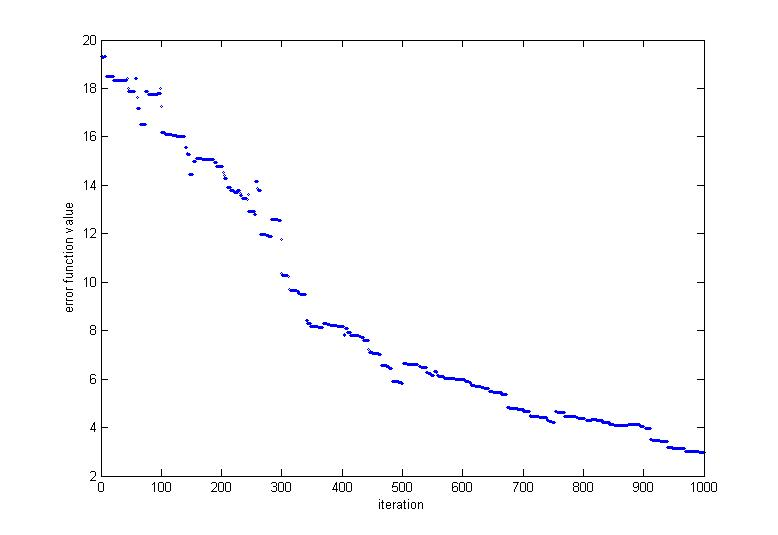
\includegraphics[width=0.9\textwidth]{ff2.jpg}\\
%\end{figure}
%}
%
%\frame{
%\frametitle{Trust region VS Newton}
%\centering
%\begin{tabular}{|r|c|c|c||r|c|c|c|}
%  \hline
%  \multicolumn{8}{|c|}{$cotoff=0.2, exact~distance, perturbation=20\%, MaxItr=150$} \\
%  \hline
%  \multicolumn{4}{|c||}{$n=200, tol=10^{-3}$} & \multicolumn{4}{c|}{$n=500, tol=10^{-2}$} \\
%  \hline
%  Alg & iter & fval & t(s) & Algo & iter & fval & t(s)\\
%  \hline
%  Alg1 & 150 & 12.234 & 40.35 & Alg1 & 150 & 167.611 & 230.60 \\
%  Alg2 & 150 &  1.234 & 38.17 & Alg2 & 150 & 221.197 & 312.59 \\
%  Alg3 & 129 &  0.531 & 26.97 & Alg3 & 150 &  11.380 & 197.97 \\
%  \hline
%  Alg1 & 150 & 11.500 & 39.91 & Alg1 & 150 & 302.333 & 222.11 \\
%  Alg2 & 150 &  5.305 & 37.93 & Alg2 & 150 & 119.509 & 273.53 \\
%  Alg3 & 150 &  0.269 & 30.68 & Alg3 & 150 &  24.185 & 186.34 \\
%  \hline
%  Alg1 & 150 & 27.146 & 37.68 & Alg1 & 150 & 273.636 & 226.34 \\
%  Alg2 & 150 &  9.764 & 36.75 & Alg2 &  93 & 188.148 & 185.29 \\
%  Alg3 & 150 &  0.365 & 30.10 & Alg3 & 150 &  49.415 & 206.23 \\
%  \hline
%\end{tabular} \\
%}
%
%\frame{
%\frametitle{Trust region VS Newton}
%\begin{figure}
%  \centering
%  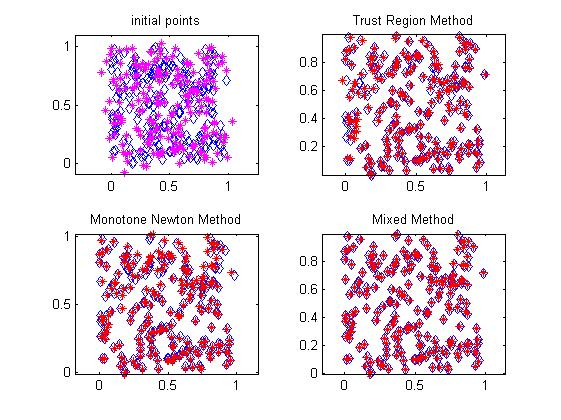
\includegraphics[width=0.9\textwidth]{TrNewton.jpg}\\
%\end{figure}
%}
%
%\frame{
%\frametitle{Trust region VS Newton}
%\begin{figure}
%  \centering
%  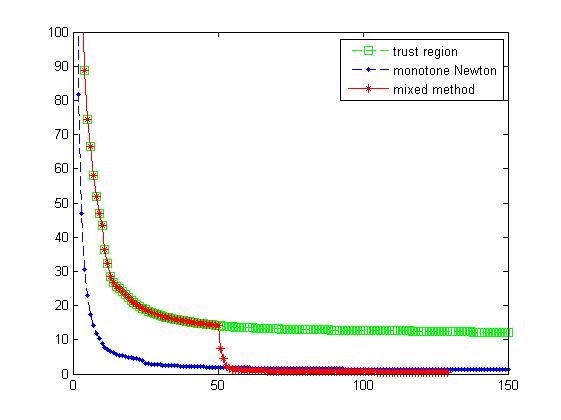
\includegraphics[width=0.7\textwidth]{TrNewtonFval.jpg}\\
%  \caption{An typical example: 200 nodes, exact distance, 20\% perturbation}
%\end{figure}
%}
%
%\frame{
%\frametitle{Trust region VS Newton}
%\begin{figure}
%  \centering
%  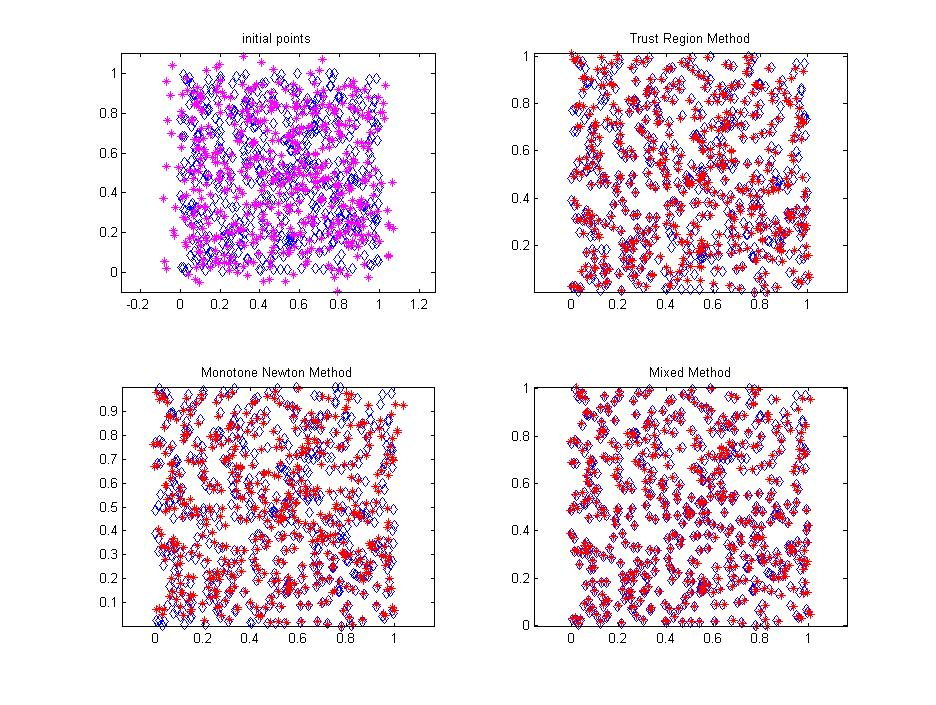
\includegraphics[width=0.9\textwidth]{TrNewton500.jpg}\\
%\end{figure}
%}
%
%\frame{
%\frametitle{Trust region VS Newton}
%\begin{figure}
%  \centering
%  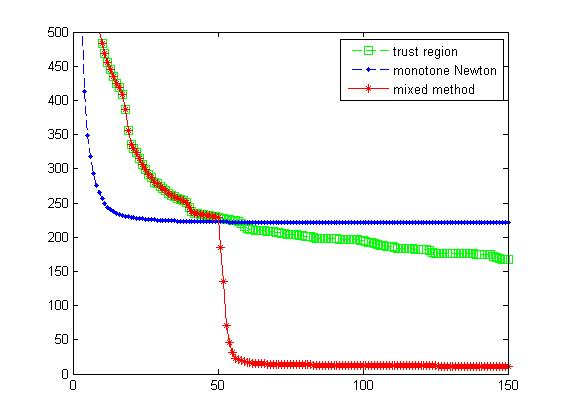
\includegraphics[width=0.7\textwidth]{TrNewtonFval500.jpg}\\
%  \caption{An typical example: 500 nodes, exact distance, 20\% perturbation}
%\end{figure}
%}
%
%\frame{
%\frametitle{Hybrid adaptively}
%\begin{figure}
%  \centering
%  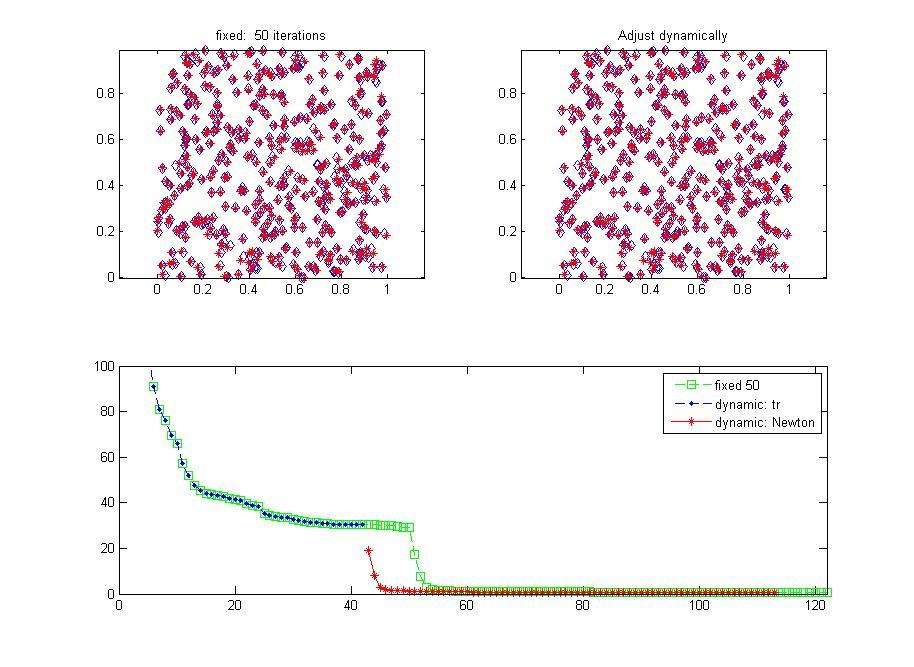
\includegraphics[width=0.65\textwidth]{dynamic.jpg}\\
%  \caption{An typical example: 200 nodes, exact distance, 20\% perturbation}
%\end{figure}
%}
%
%\frame{
%\frametitle{Hybrid adaptively}
%\begin{center}
%\begin{tabular}{|c|c|c|c|c|}
%  \hline
%  method  & k' & iter & fval  & time  \\
%  \hline
%  fixed   & 50 &  122 & 0.789 & 25.06 \\
%  dynamic & 42 &  113 & 0.671 & 23.49 \\
%  \hline
%\end{tabular}
%\end{center}
%\vspace{0.5cm}
%\begin{description}
%  \item[set up:] 200 nodes, cutoff=0.2, exact distances, 20\% perturbation, {\red $tol=10^{-3}$}. switch criterion: k=min\{50, k'\}, where k' is the smallest number such that $$fval(i-1)-fval(i)<{\red 100}*tol.$$
%\end{description}
%\begin{itemize}
%  \item Performance differ slightly with different parameters, usually is not worse that fixed method.
%\end{itemize}
%}
%
%\frame{
%\frametitle{exact VS noise distances}
%\centering
%\begin{tabular}{|r|c|c|c||r|c|c|c|}
%  \hline
%  \multicolumn{8}{|c|}{$cotoff=0.2, perturbation=20\%, MaxItr=150, tol=10^{-3}$} \\
%  \hline
%  \multicolumn{4}{|c||}{$n=200, noise=1\%$} & \multicolumn{4}{c|}{$n=200, noise=5\%$} \\
%  \hline
%  dist & iter & fval & t(s) & dist & iter & fval & t(s)\\
%  \hline
%  exact & 150 &  1.548 & 30.52 & exact & 150 &  0.111 & 31.22 \\
%  noise & 150 &  0.304 & 30.64 & noise & 150 &  1.665 & 30.93 \\
%  \hline
%  exact & 137 &  0.137 & 29.65 & exact & 148 &  1.060 & 29.94 \\
%  noise & 136 &  0.677 & 30.55 & noise & 150 &  1.167 & 30.32 \\
%  \hline
%  \multicolumn{4}{|c||}{$n=200, noise=10\%$} & \multicolumn{4}{c|}{$n=200, noise=20\%$} \\
%  \hline
%  exact & 143 &  0.037 & 30.05 & exact & 143 &  0.420 & 28.71 \\
%  noise & 150 &  0.734 & 31.07 & noise & 150 &  5.265 & 30.06 \\
%  \hline
%  exact & 150 &  0.516 & 29.57 & exact & 109 &  0.057 & 22.83 \\
%  noise & 150 &  2.134 & 29.68 & noise &  77 &  5.068 & 18.23 \\
%  \hline
%\end{tabular} \\ }
%
%\frame{
%\frametitle{Trust region VS Newton}
%\begin{figure}
%  \centering
%  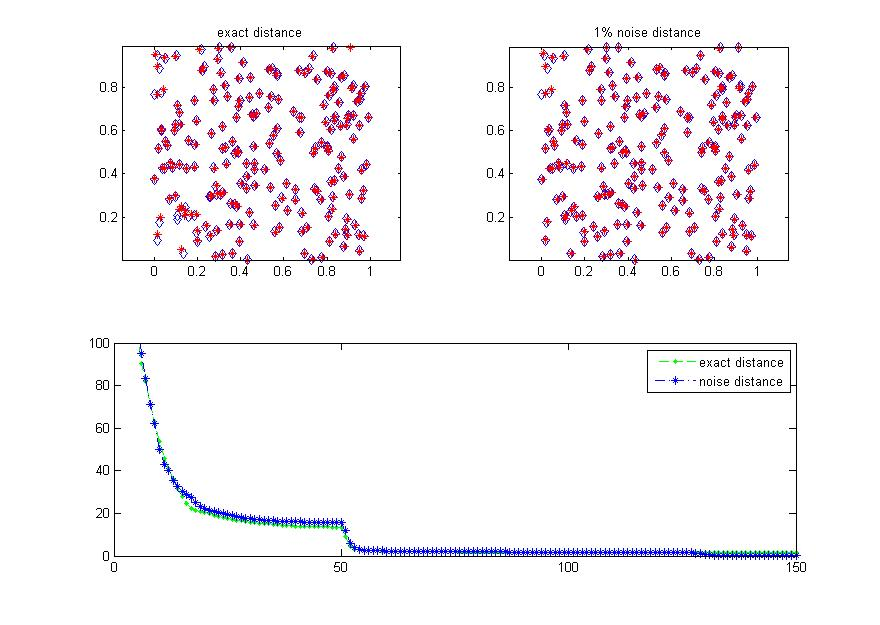
\includegraphics[width=0.9\textwidth]{noise1.jpg}\\
%  %\caption{An typical example of graph with 200 nodes, 1\% noise distance}
%\end{figure}
%}
%
%\frame{
%\frametitle{Trust region VS Newton}
%\begin{figure}
%  \centering
%  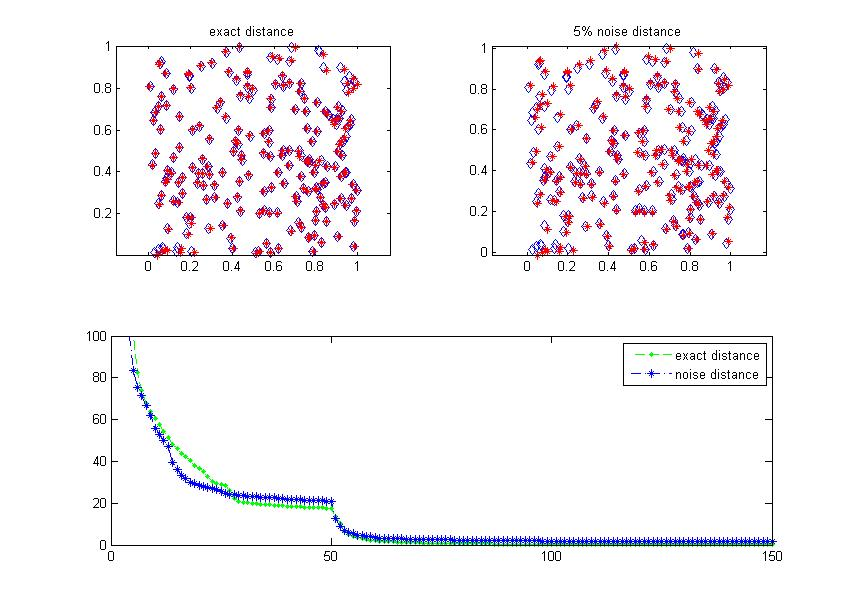
\includegraphics[width=0.9\textwidth]{noise5.jpg}\\
%  %\caption{An typical example of graph with 200 nodes, 5\% noise distance}
%\end{figure}
%}
%
%\frame{
%\frametitle{Trust region VS Newton}
%\begin{figure}
%  \centering
%  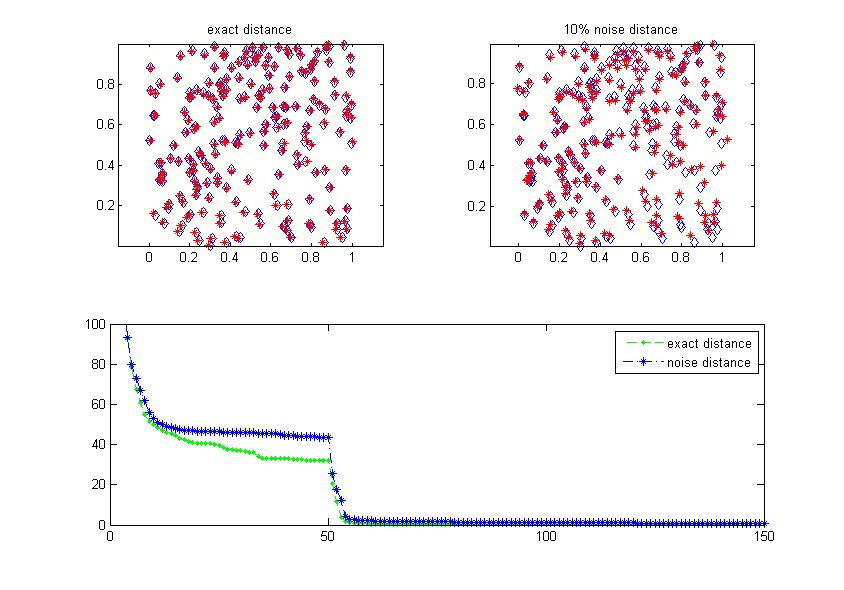
\includegraphics[width=0.9\textwidth]{noise10.jpg}\\
%  %\caption{An typical example of graph with 200 nodes, 10\% noise distance}
%\end{figure}
%}
%
%\frame{
%\frametitle{Trust region VS Newton}
%\begin{figure}
%  \centering
%  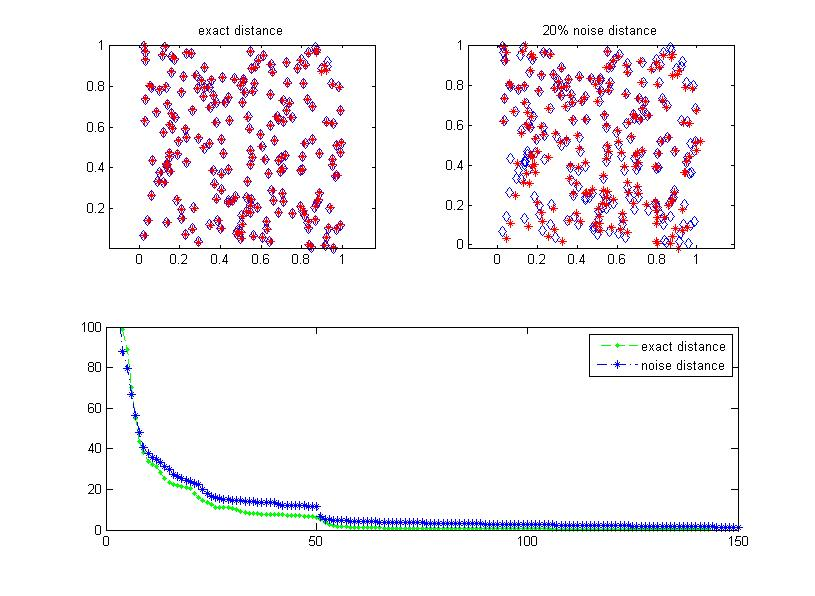
\includegraphics[width=0.9\textwidth]{noise20.jpg}\\
%  %\caption{An typical example of graph with 200 nodes, 20\% noise distance}
%\end{figure}
%}
%
%\section{Conclusions and ongoing works}
%
%\frame{
%\frametitle{A generalized DG problem}
%{\red DG problem with distance bounds}  \\
%\textrm{}\\
%Given the lower bounds $l_{i,j}$ and upper bounds $u_{i,j}$, the problem can be formulated as (Sit-Wu-2011):
%\begin{align*}
%  \max_{x_{i},r_{i}} \quad & \sum_{i=1}^{n} r_{i} \\
%  \st                \quad & \|x_{i}-x_{j}\|+r_{i}+r_{j}\leq u_{i,j} \\
%                           & \|x_{i}-x_{j}\|-r_{i}-r_{j}\geq l_{i,j} \qquad \forall (i,j)\in S\\
%                           &  r_{i}\geq 0, \qquad i=1,2,\ldots,n.
%\end{align*}
%%\footnotesize{Atilla Sit, Zhijun Wu(2011), {\blue Solving a Generalized Distances Geometry Problem for Protein Structure Determination. }}
%}
%
%\frame{
%\frametitle{??? Gradient calculation}
%I try to write the problem in a compact form (in matrix/vector).\\
%Define the coefficient matrix $A\in \mathbb{R}^{|S|\times n}$, for example (a clique with four points)
%$$A=\left( \begin{array}{cccc}
%             1 & -1 & 0 & 0 \\
%             1 & 0 & -1 & 0 \\
%             1 & 0 & 0 & -1 \\
%             0 & 1 & -1 & 0 \\
%             0 & 1 & 0 & -1 \\
%             0 & 0 & 1 & -1 \\
%           \end{array} \right)
%$$
%and $X=(x_{1},x_{2},\ldots,x_{n}\Tran)$, $d=(d_{ij})$ which is a column vector, then
%$$AX=\left( \begin{array}{c}
%              \cdots \\
%              x_{i}-x_{j} \\
%              \cdots
%            \end{array}
%\right).$$
%Then ??? $\ldots\ldots$ {\red The problem is that $x_{i}$ is a vector, rather than a scalar}.
%}
%
%\frame{
%\frametitle{how to compare functions?}
%\begin{itemize}
%  \item is it possible to "count" how many local minimizers a function have (even though roughly)?
%  \item numerical ways?
%  \item figure intuition?
%\end{itemize}
%}
%
%\frame{
%\begin{figure}
%  \centering
%  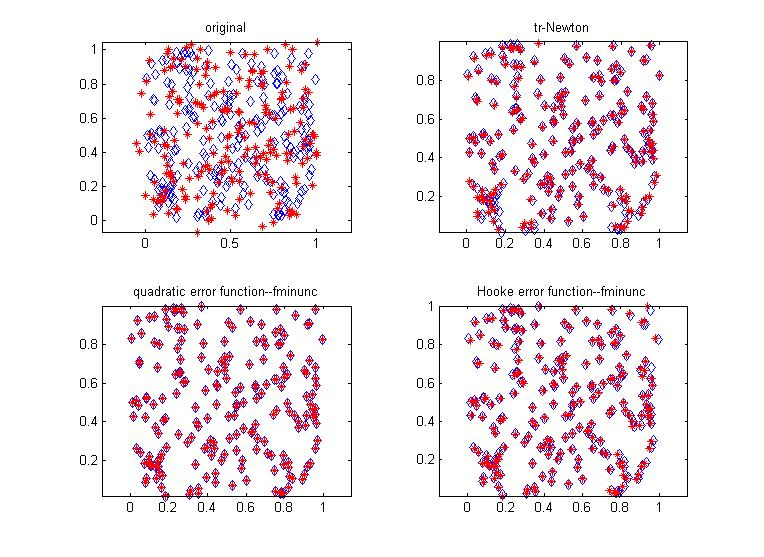
\includegraphics[width=\textwidth]{testErrorFunc.jpg}\\
%\end{figure}
%
%\frametitle{}
%}
%
%\frame{
%\frametitle{Conclusions and Future work}
%\begin{itemize}%[$\blacktriangleright$]
%  \item What we have done:
%        \begin{enumerate}[--]
%          \item proposed a novel error function
%          \item based on the proposed function, designed an efficient algorithm to solve the distance geometry problem
%          \item finished some preliminary numerical experiments, which seems promising, especially in the noise case
%        \end{enumerate}
%  \item Future work:
%        \begin{enumerate}[--]
%          \item theoretical convergence analysis of the algorithm
%          \item generalize the error function to handle the "bound" case
%          \item compare the algorithm with the existing ones
%        \end{enumerate}
%\end{itemize}
%}
%
%
\frame{
%\frametitle{Q \& A}
\begin{center}
  \Large{  \textsc{Thank you for your attention!}}  \\
  \vspace{0.2cm}
  {\blue szl@lsec.cc.ac.cn }
\end{center}
}

\end{CJK*}
\end{document}
